\section{RESULTADOS}

Os resultados apresentados a seguir correspondem ao modelo SNN ajustado com
aumento de dados (fator 5, ruído gaussiano leve) e seleção de hiperparâmetros
via busca em grade. As análises exploratórias mostram a distribuição das
variáveis e suas correlações, enquanto as figuras de desempenho destacam a
estabilidade do treinamento e a qualidade das predições em relação aos valores
observados.

Após a busca em grade, a melhor configuração encontrada foi: $hidden\_size=64$,
$time\_steps=15$, $lr=0{,}002$, $\beta=0{,}95$, $thresh=0{,}8$ e ruído de aumento
$\sigma=0{,}02$, com parada antecipada por paciência de 20 épocas. Com essa
configuração, o modelo final atingiu desempenho de teste com $MSE=0{,}0327$ e
$MAE=0{,}1437$ para a predição de pH. Considerando a faixa observada de pH no
conjunto (aprox. 5{,}16 a 6{,}52), o erro médio absoluto representa uma fração
reduzida do intervalo total, indicando boa precisão relativa para um conjunto
de dados pequeno. A Figura~\ref{fig:pred_pH} evidencia a proximidade entre valores
preditos e reais, enquanto a Figura~\ref{fig:hist_loss} mostra convergência
rápida e estável do treinamento.

Também foi treinado um modelo multimodal (multi-saída) para prever simultaneamente
pH, OD e turbidez. O melhor ajuste multimodal apresentou, no conjunto de teste,
as seguintes métricas: $MAE_{pH}=0{,}115$, $MAE_{OD}=0{,}072$ e $MAE_{TURB}=0{,}392$,
com $R^{2}_{pH}=0{,}723$, $R^{2}_{OD}=0{,}908$ e $R^{2}_{TURB}=0{,}909$. Esses valores
indicam bom desempenho para pH e OD, e desempenho aceitável para turbidez. As
Figuras~\ref{fig:multi_pred} e \ref{fig:multi_res} apresentam as predições e
os resíduos do modelo multimodal, respectivamente.

\begin{figure}[ht!]
	\centering
	\begin{minipage}{0.48\textwidth}
		\centering
		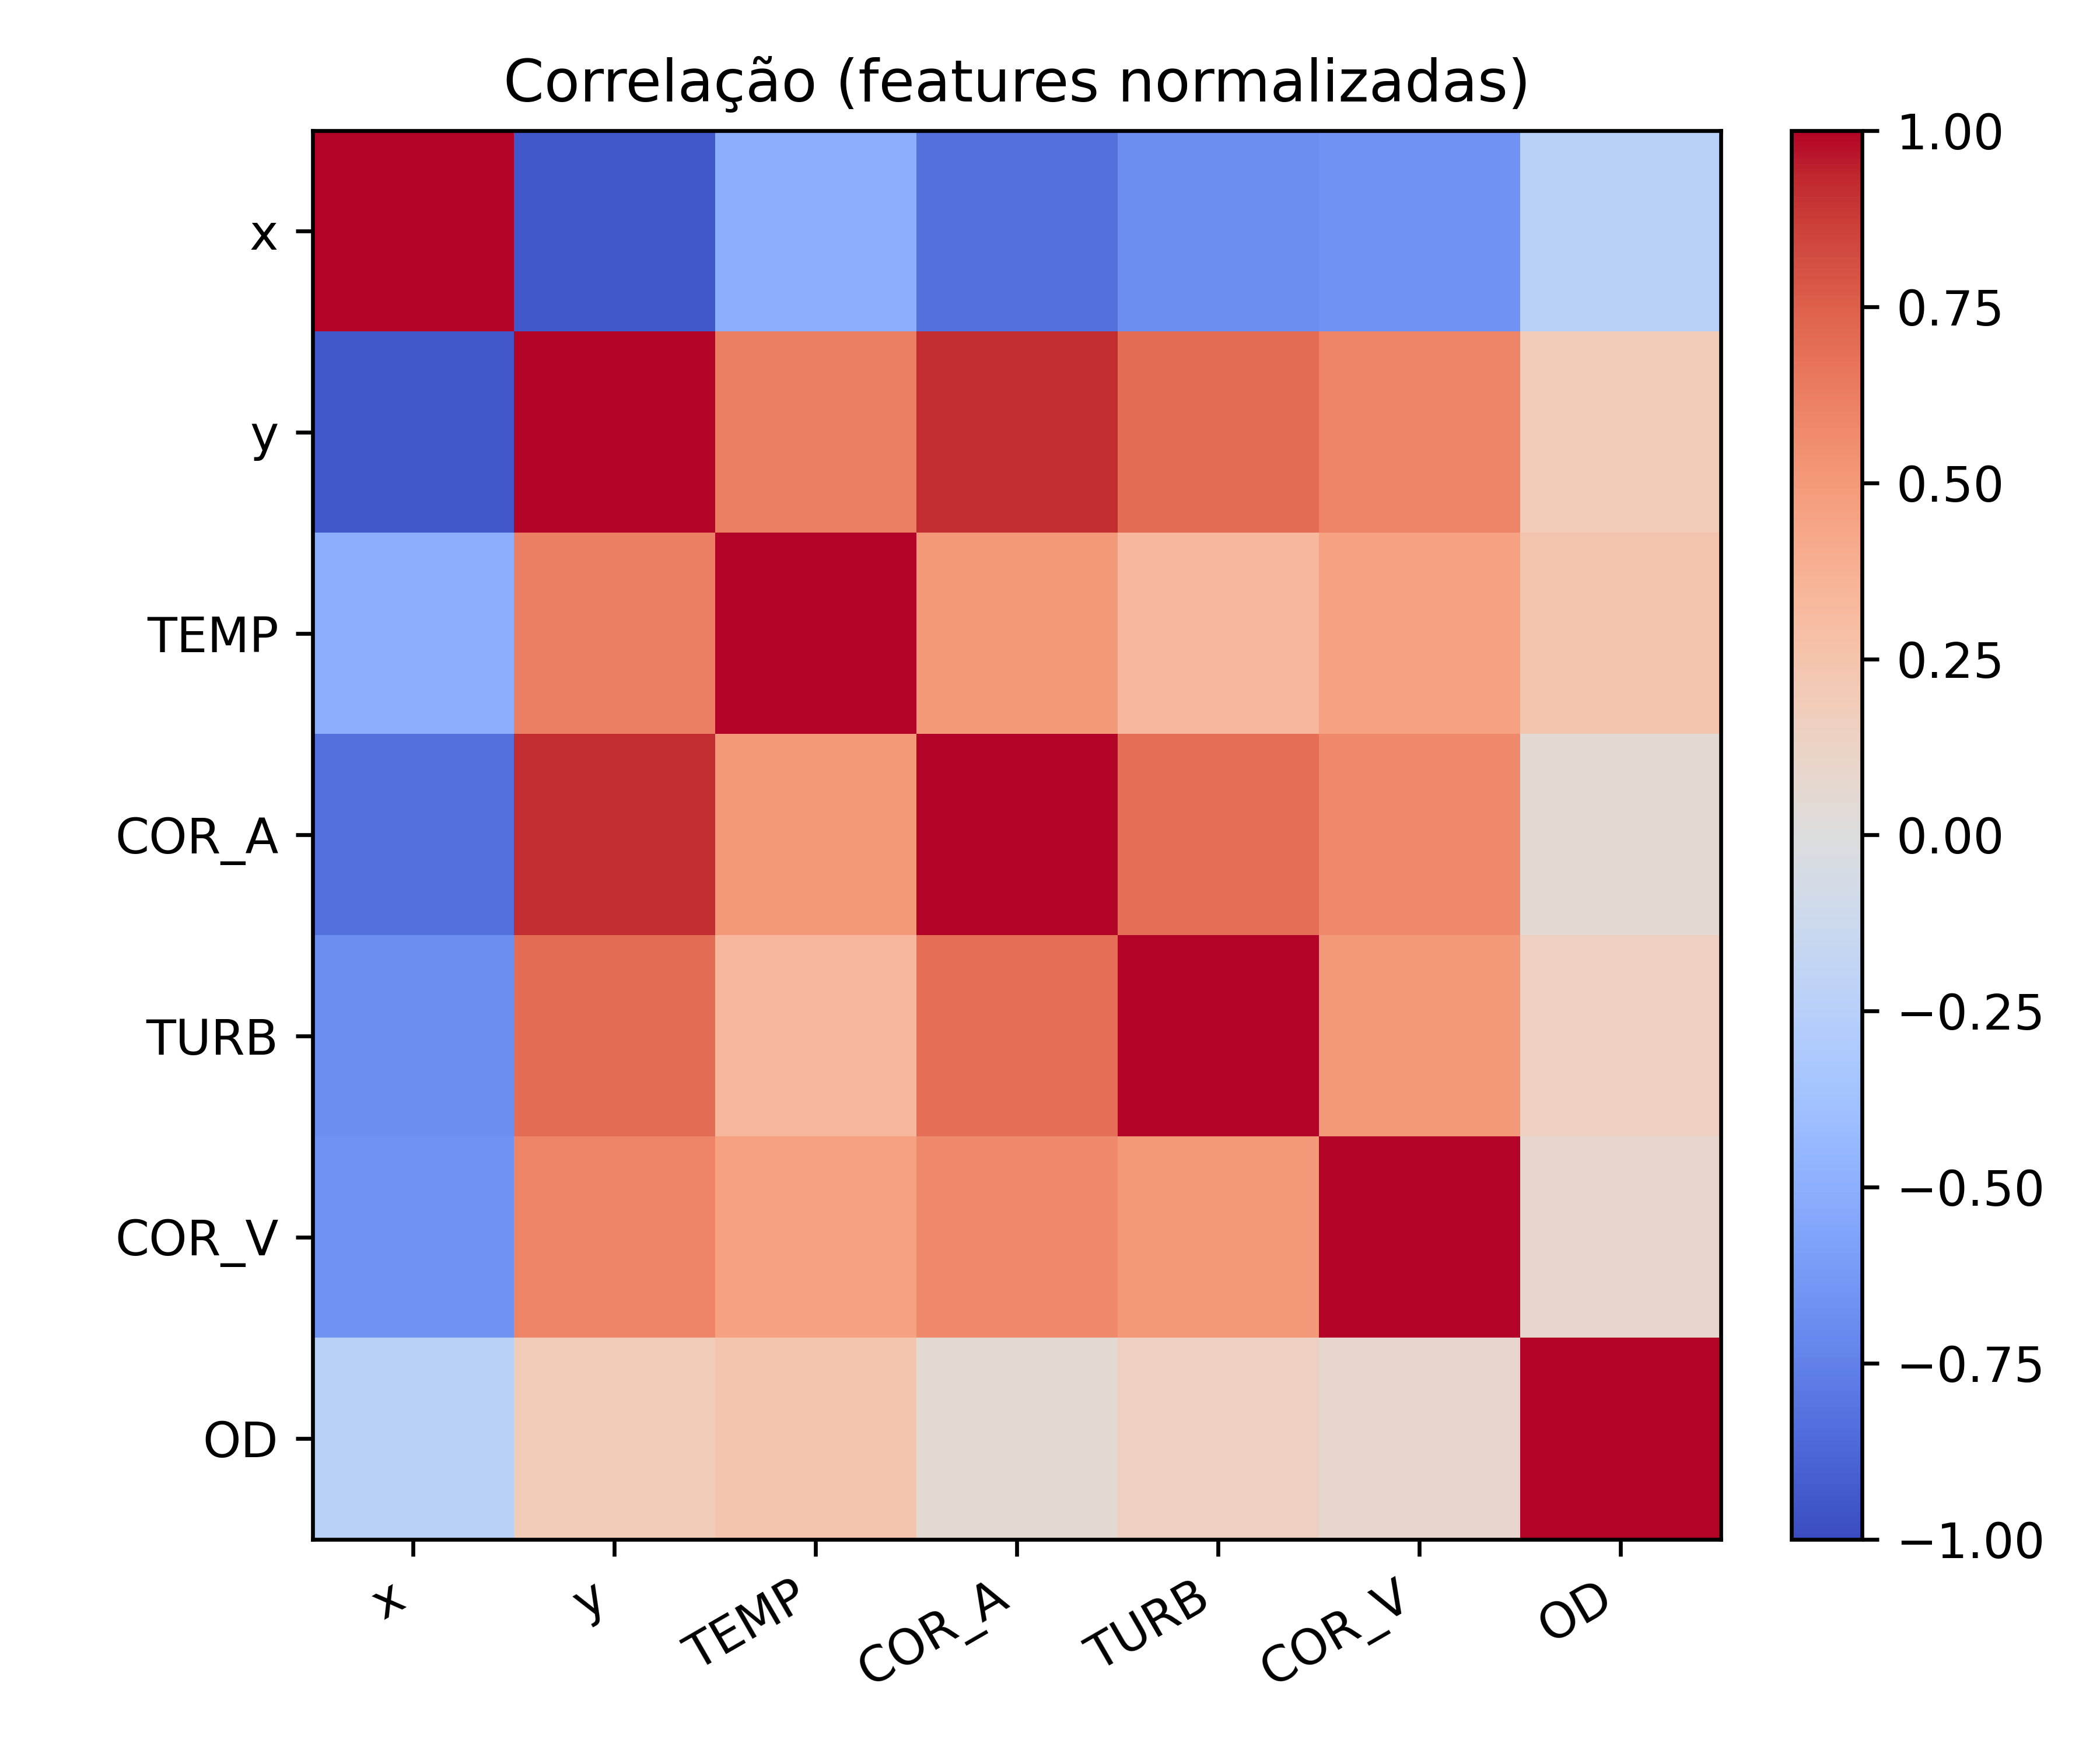
\includegraphics[width=\linewidth]{./figuras/corr_heatmap.png}
		\caption*{(a) Correlação entre variáveis}
	\end{minipage}\hfill
	\begin{minipage}{0.48\textwidth}
		\centering
		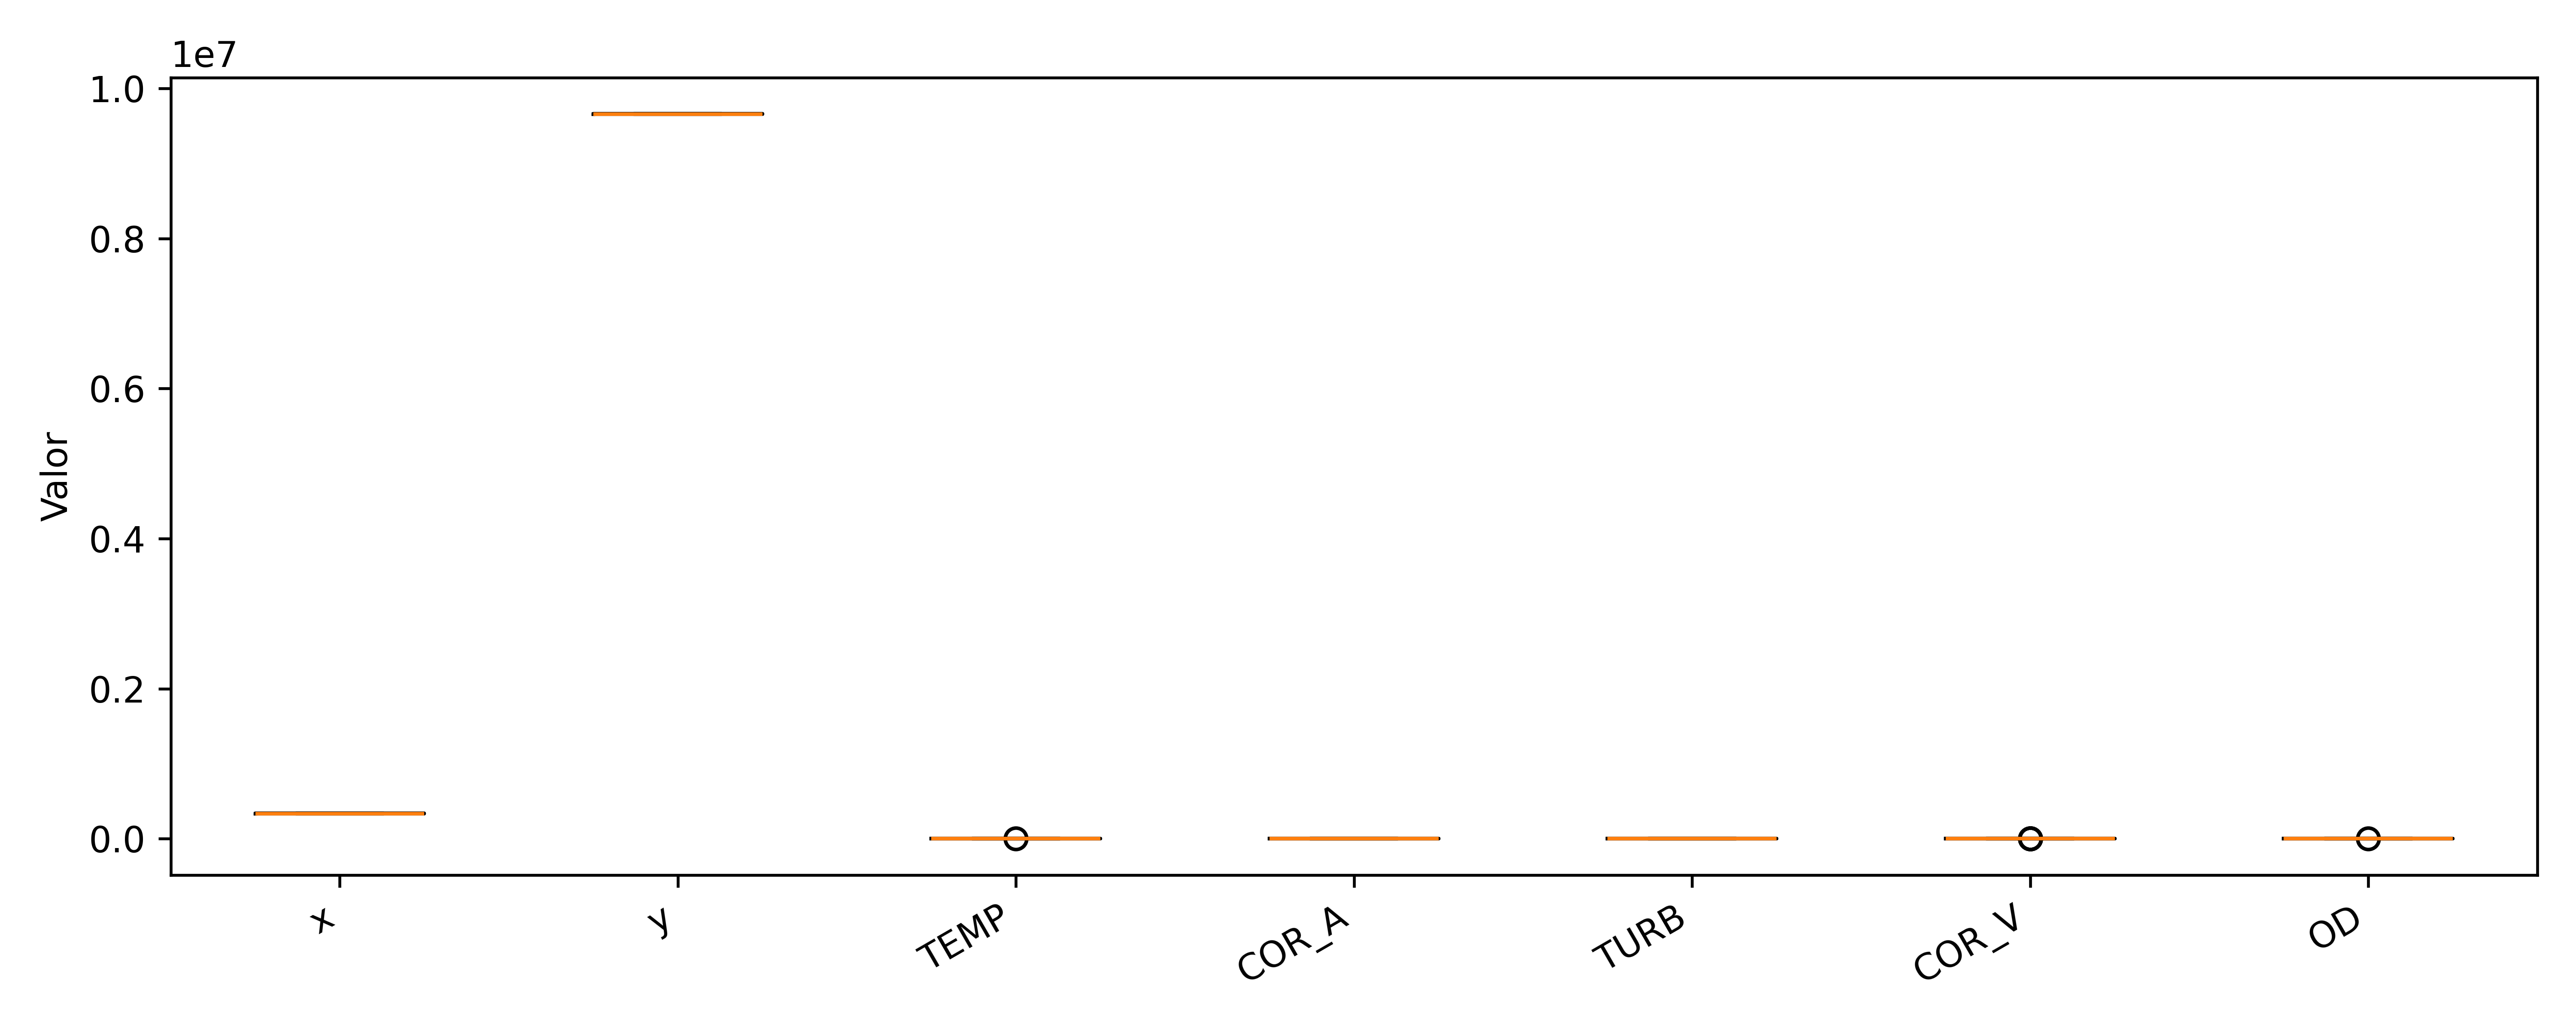
\includegraphics[width=\linewidth]{./figuras/boxplots_features.png}
		\caption*{(b) Boxplots das variáveis}
	\end{minipage}
	\caption{Análise exploratória: correlações e distribuição das variáveis de entrada.}
	\label{fig:exploratoria}
\end{figure}

As Figuras~\ref{fig:exploratoria} e \ref{fig:hist_loss} sintetizam a etapa exploratória. O mapa de
correlação indica relações entre variáveis ambientais, enquanto os boxplots mostram dispersão e
possíveis outliers. Essas informações orientam a interpretação dos modelos e ajudam a contextualizar
as variações observadas nos parâmetros físico-químicos.

\begin{figure}[ht!]
	\centering
	\begin{minipage}{0.48\textwidth}
		\centering
		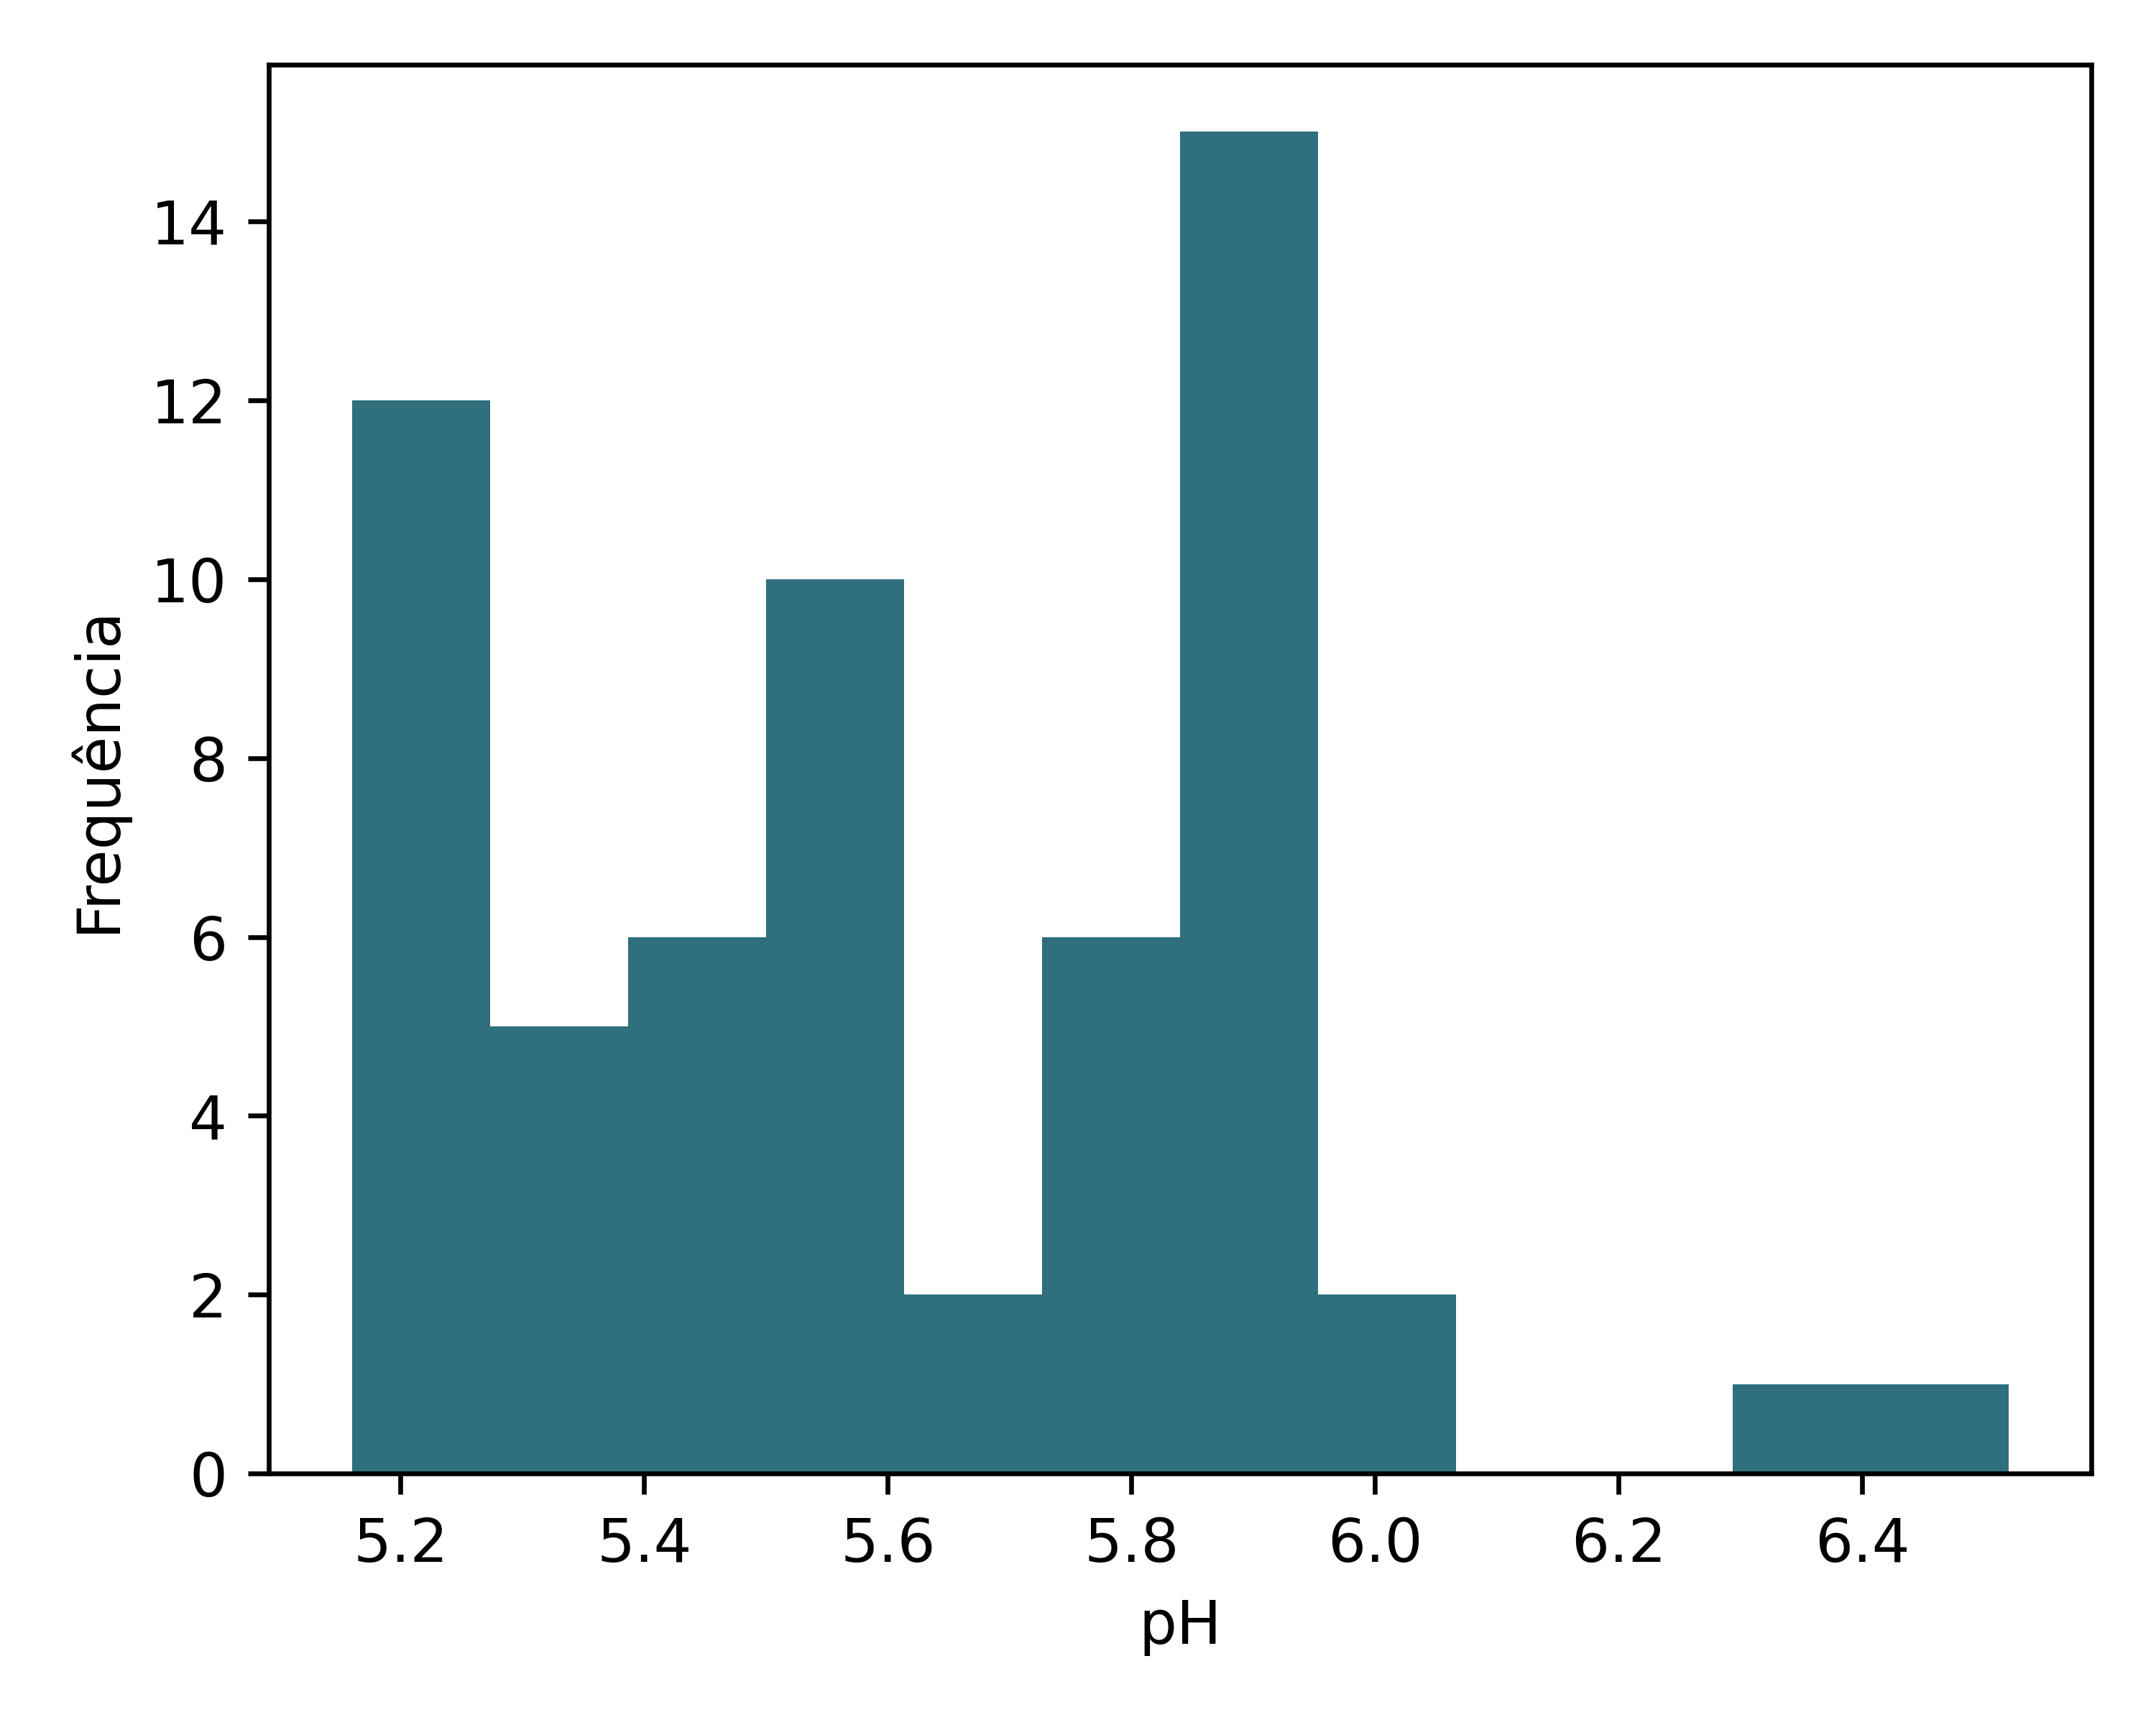
\includegraphics[width=\linewidth]{./figuras/hist_pH.png}
		\caption*{(a) Histograma do pH}
	\end{minipage}\hfill
	\begin{minipage}{0.48\textwidth}
		\centering
		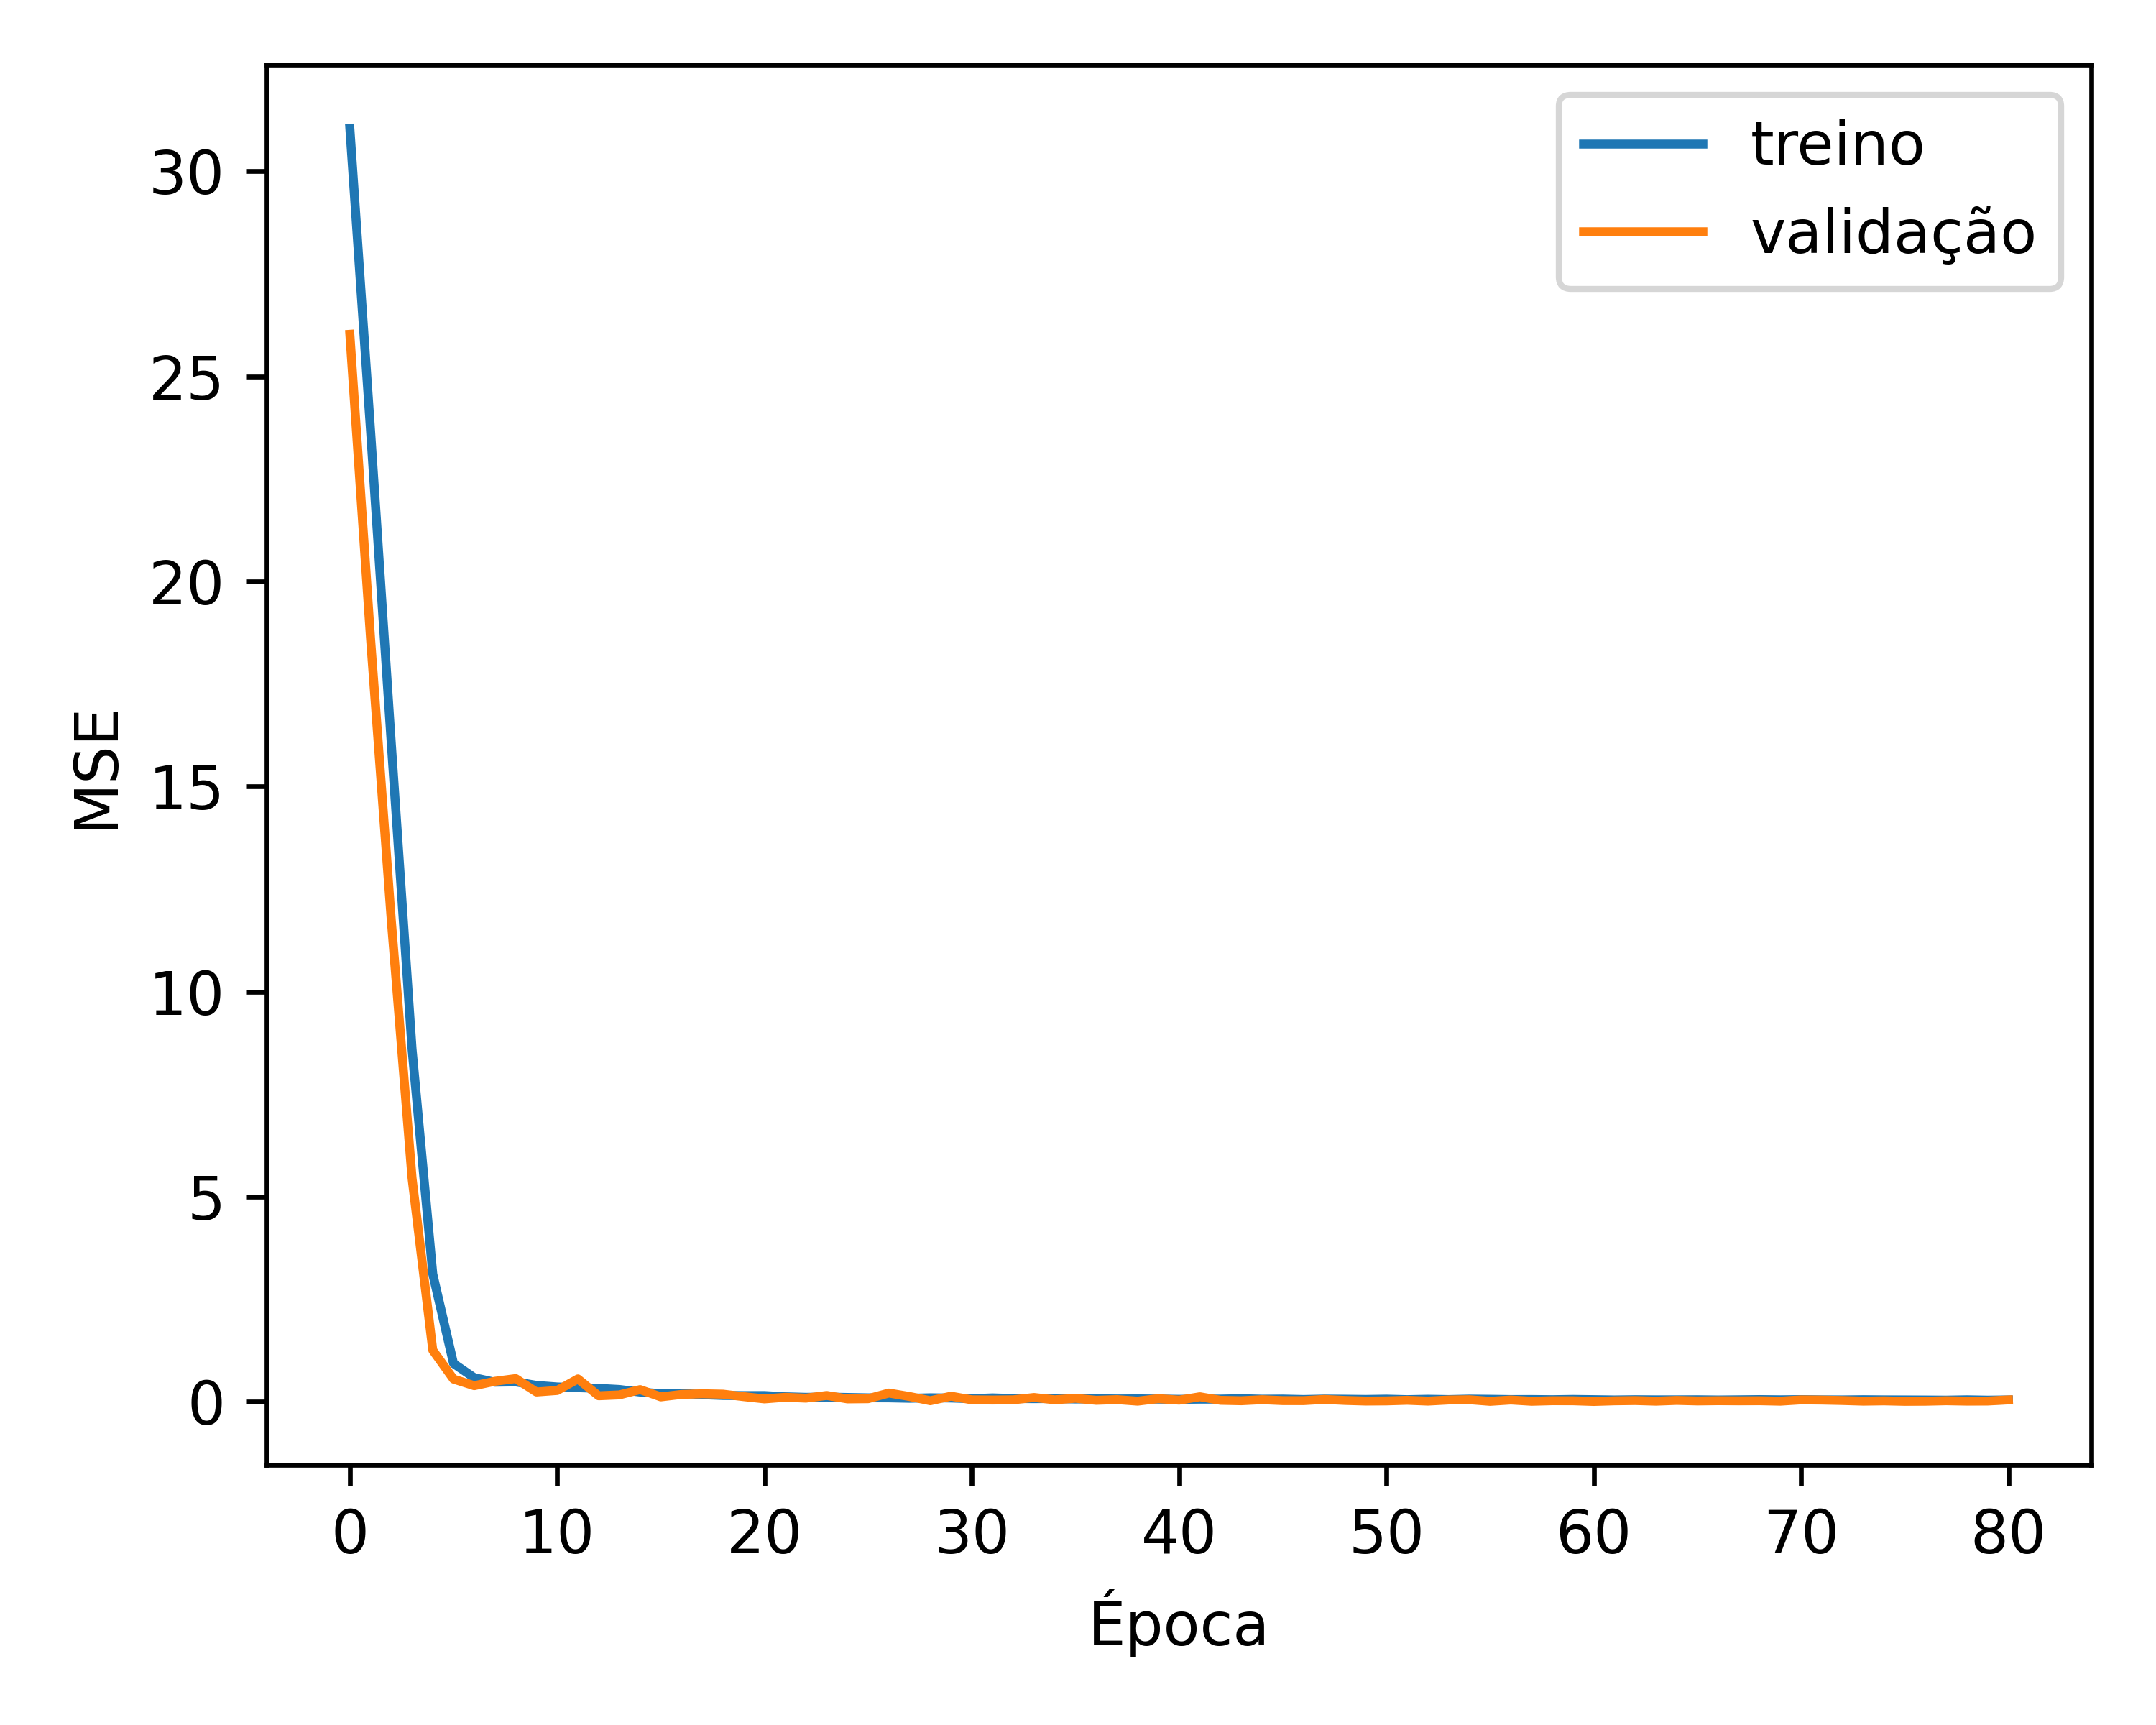
\includegraphics[width=\linewidth]{./figuras/loss_curve.png}
		\caption*{(b) Curva de perda (MSE)}
	\end{minipage}
	\caption{Distribuição do alvo e dinâmica de treinamento/validação.}
	\label{fig:hist_loss}
\end{figure}

O histograma do pH evidencia a concentração de valores em uma faixa estreita, o que reforça a
necessidade de modelos sensíveis a pequenas variações. A curva de perda mostra convergência rápida
e estável, compatível com o uso de \textit{early stopping}.

\begin{figure}[ht!]
	\centering
	\begin{minipage}{0.48\textwidth}
		\centering
		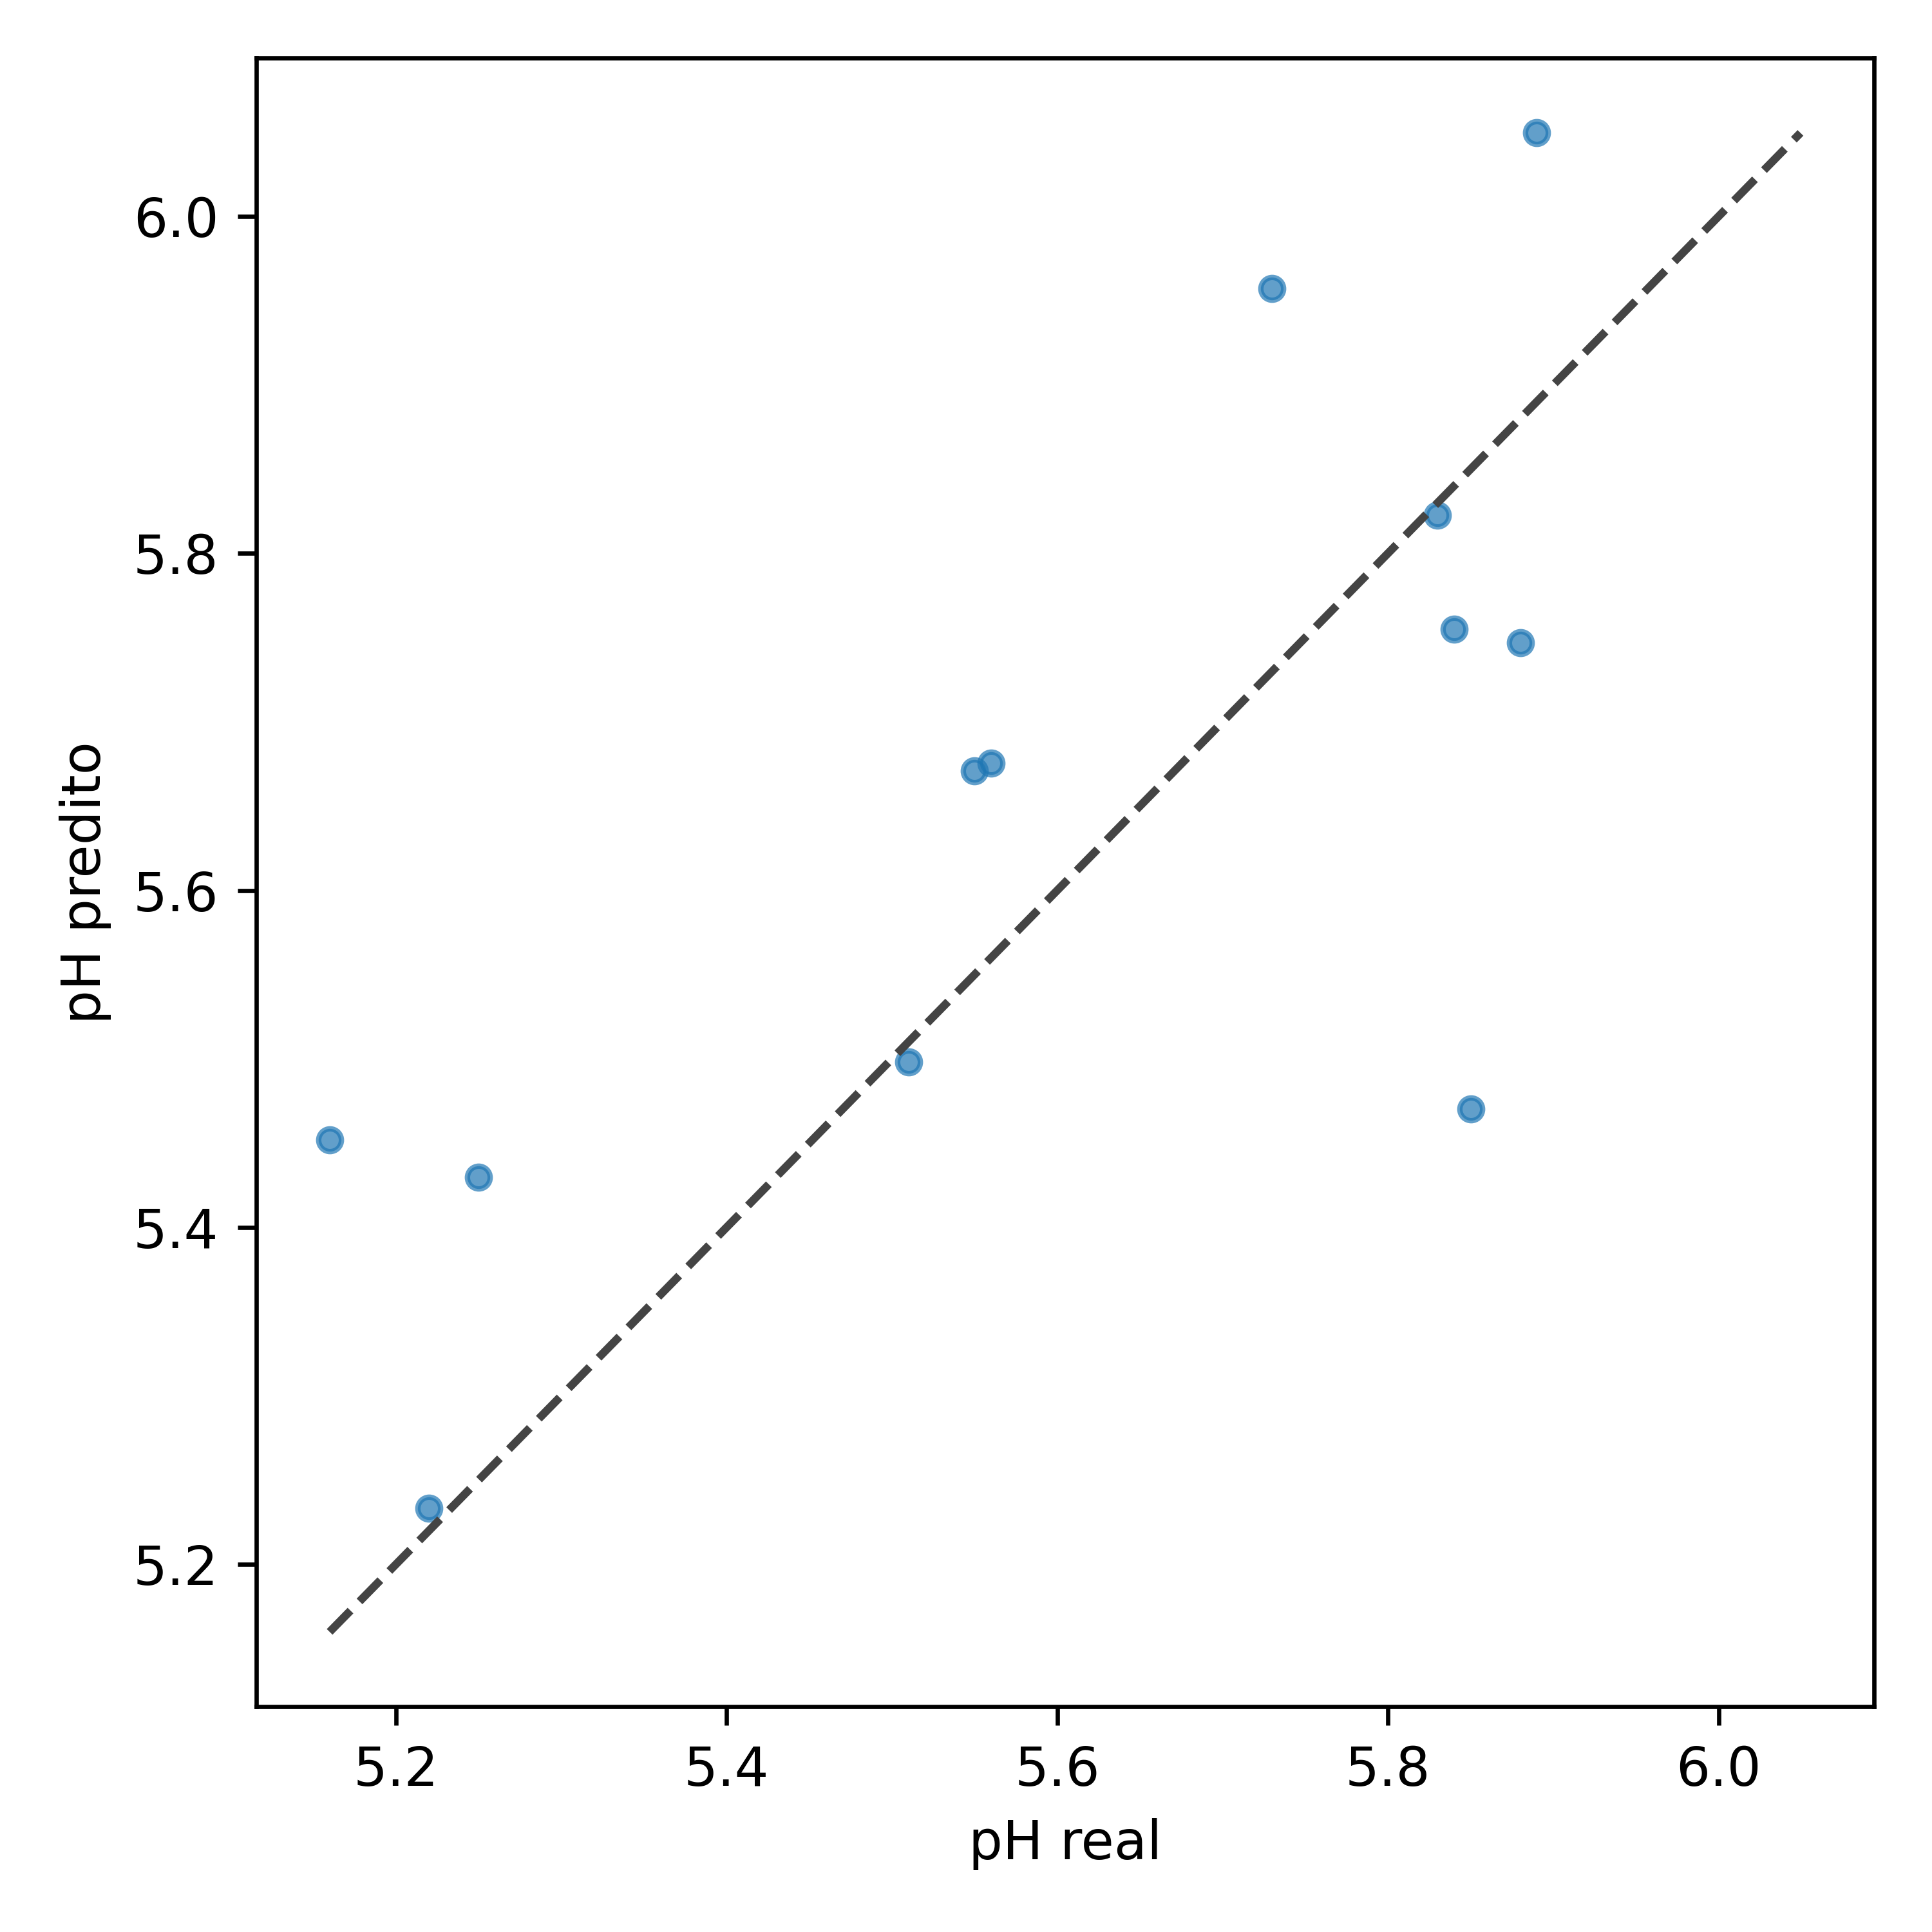
\includegraphics[width=\linewidth]{./figuras/pred_vs_real_pH.png}
		\caption*{(a) Predito vs. real}
	\end{minipage}\hfill
	\begin{minipage}{0.48\textwidth}
		\centering
		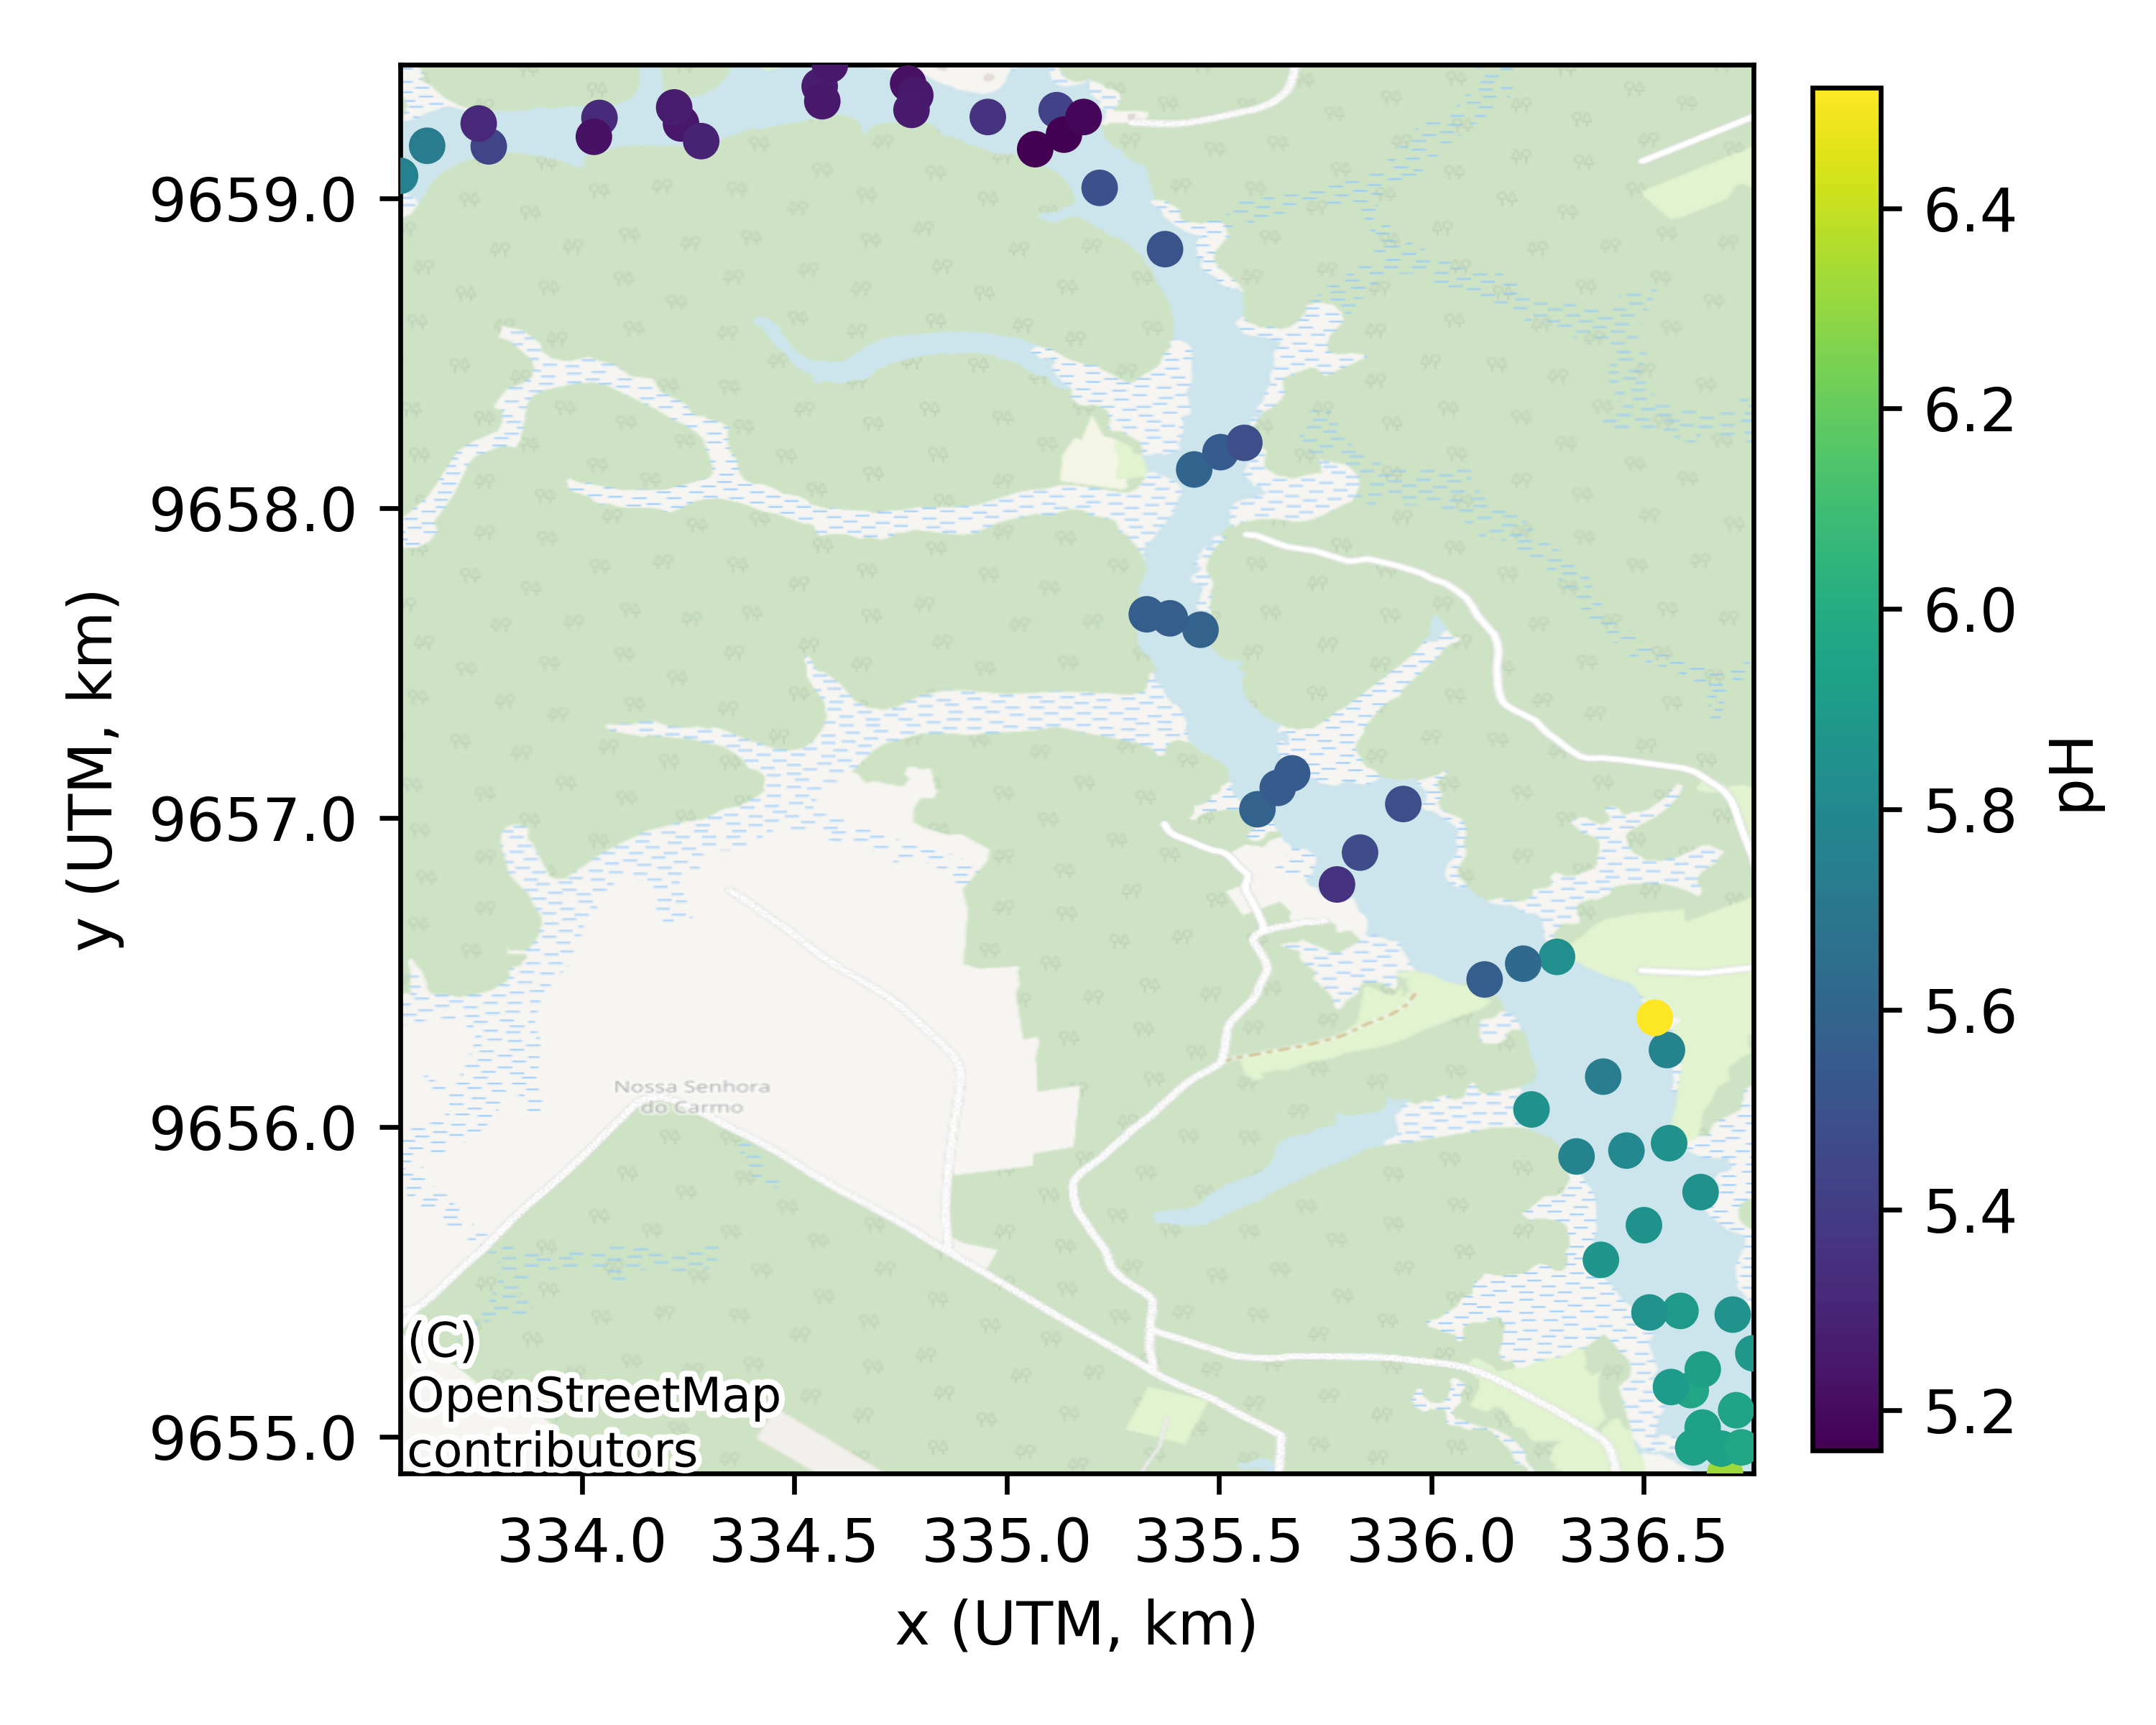
\includegraphics[width=\linewidth]{./figuras/map_pH.png}
		\caption*{(b) Mapa espacial de pH}
	\end{minipage}
	\caption{Desempenho preditivo e padrão espacial do pH no Lago do Serpa.}
	\label{fig:pred_pH}
\end{figure}

Na Figura~\ref{fig:pred_pH}, a proximidade dos pontos à linha de identidade indica boa capacidade
do modelo em reproduzir o pH observado. O mapa espacial do pH revela gradientes coerentes no lago,
com regiões de valores mais elevados concentradas em setores específicos.

\begin{figure}[ht!]
	\centering
	\begin{minipage}{0.48\textwidth}
		\centering
		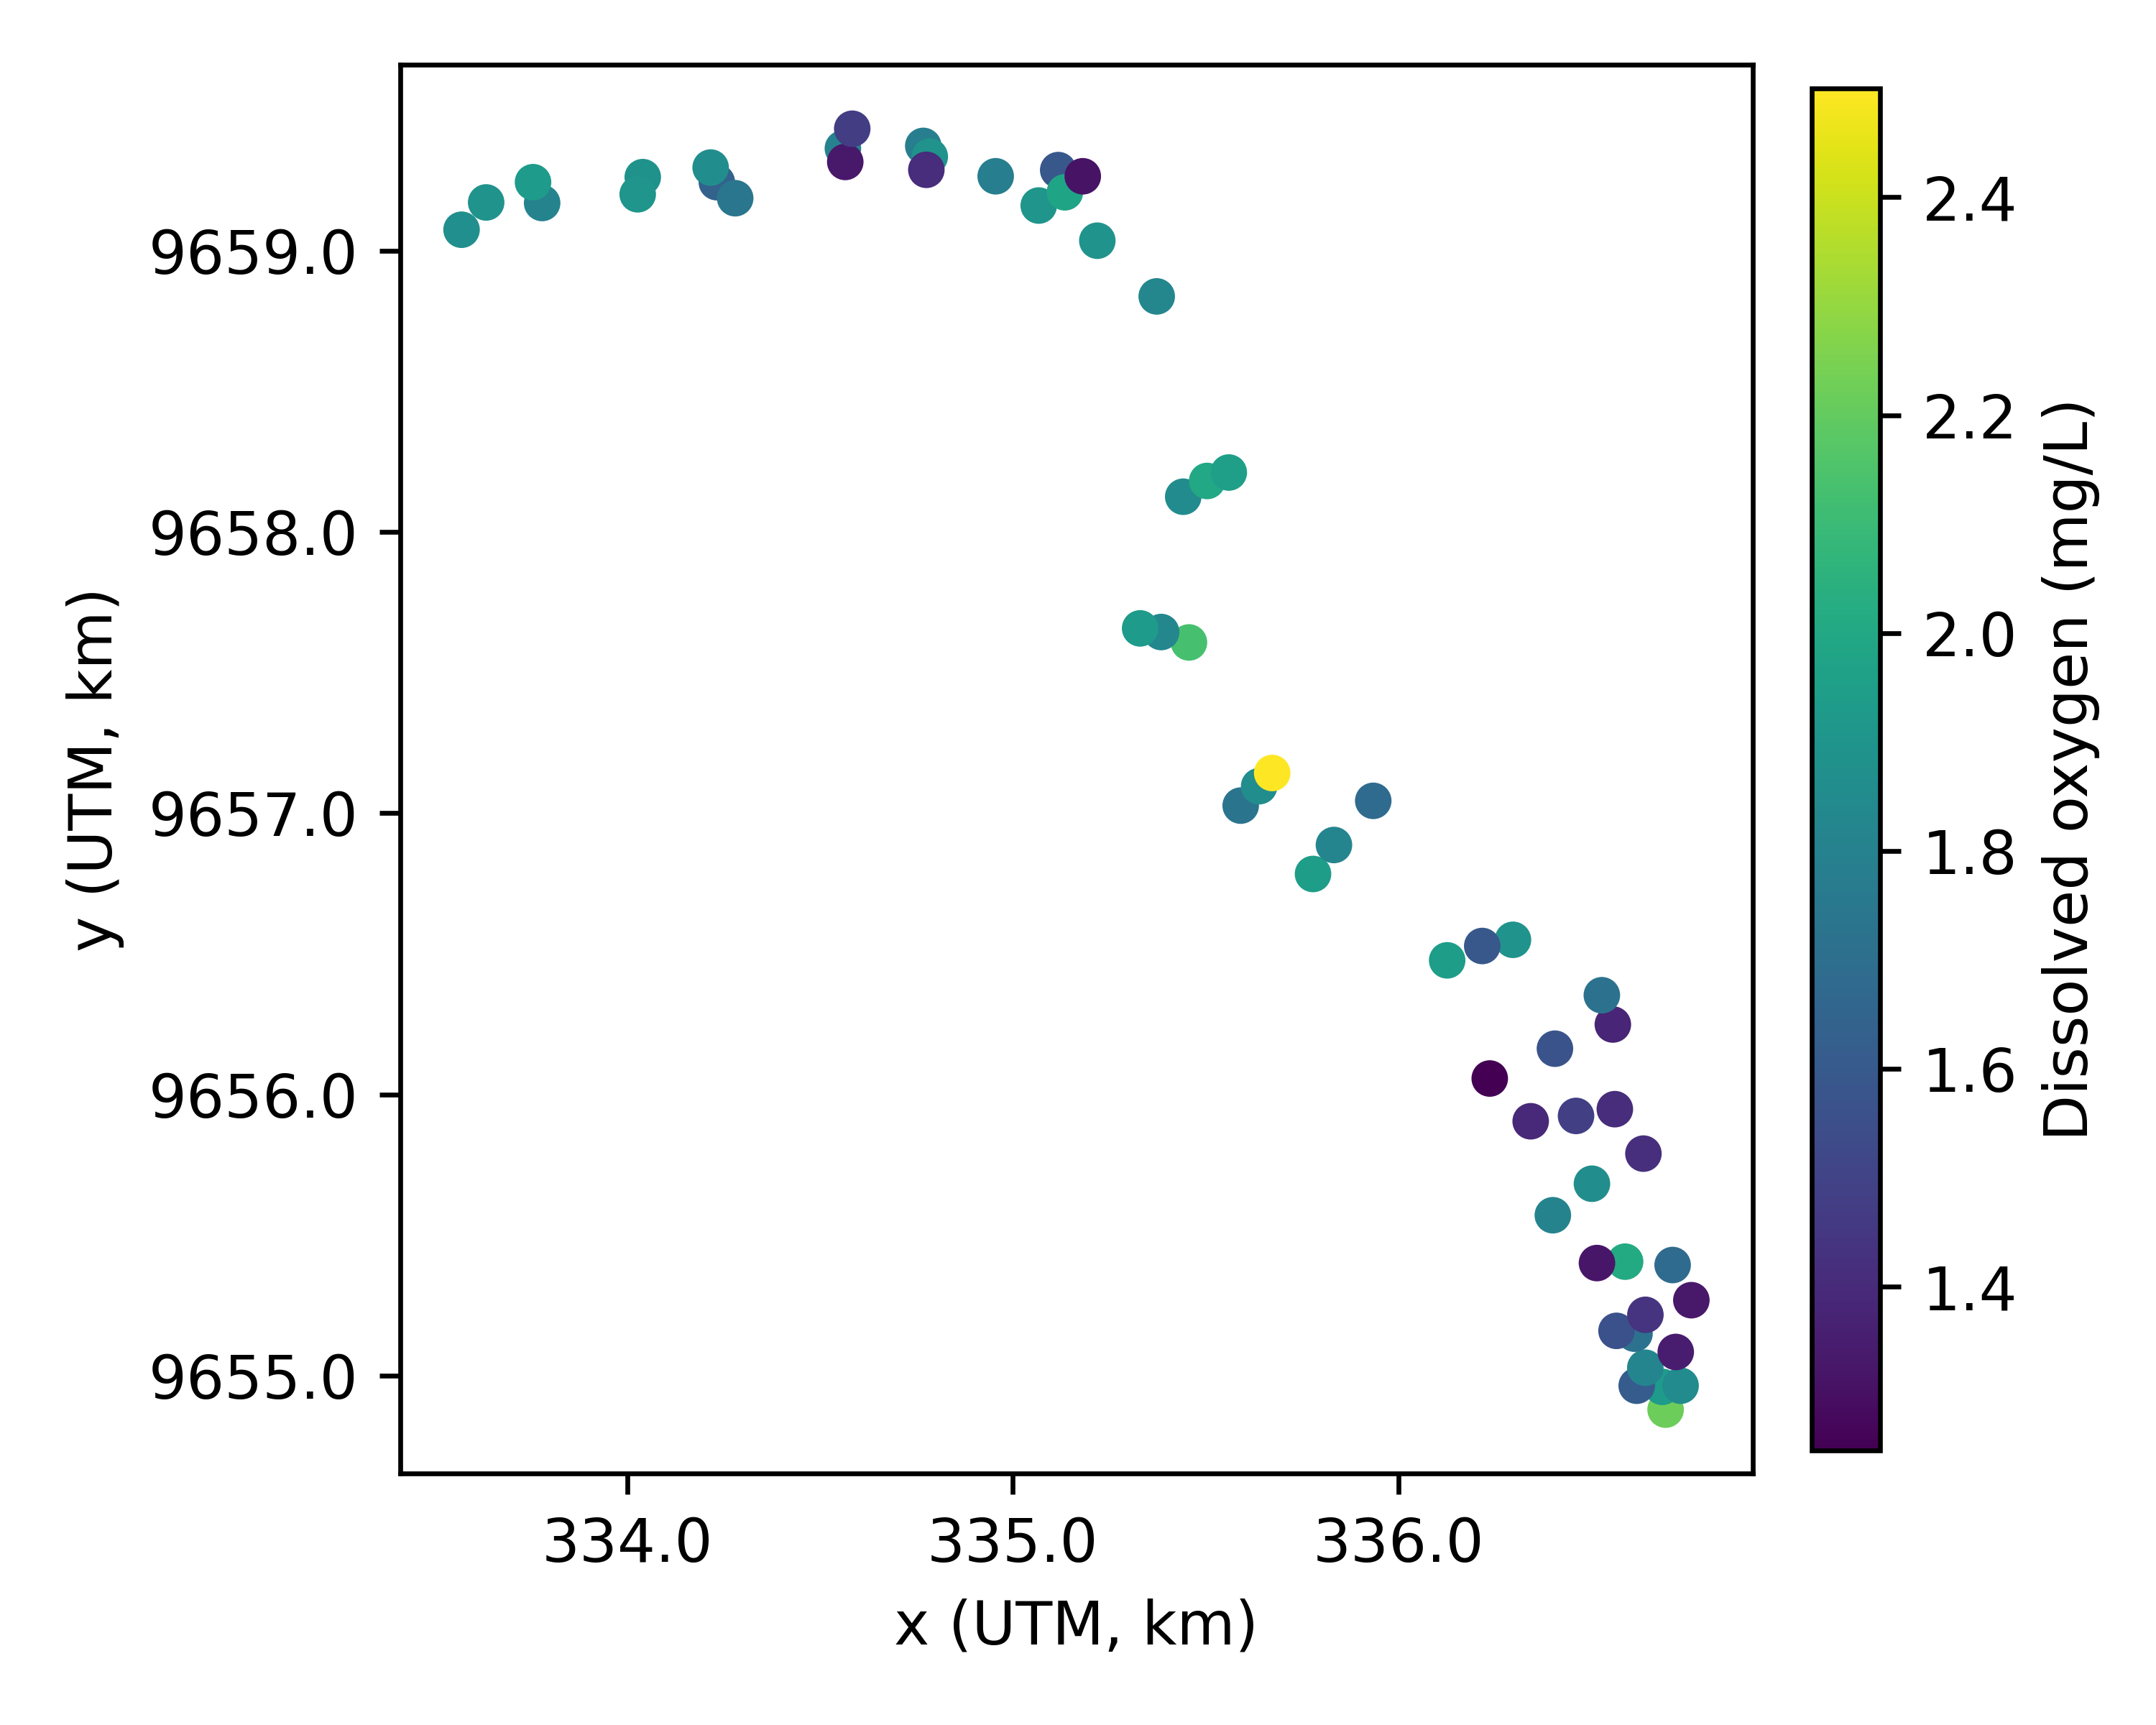
\includegraphics[width=\linewidth]{./figuras/map_OD.png}
		\caption*{(a) Mapa espacial de OD}
	\end{minipage}\hfill
	\begin{minipage}{0.48\textwidth}
		\centering
		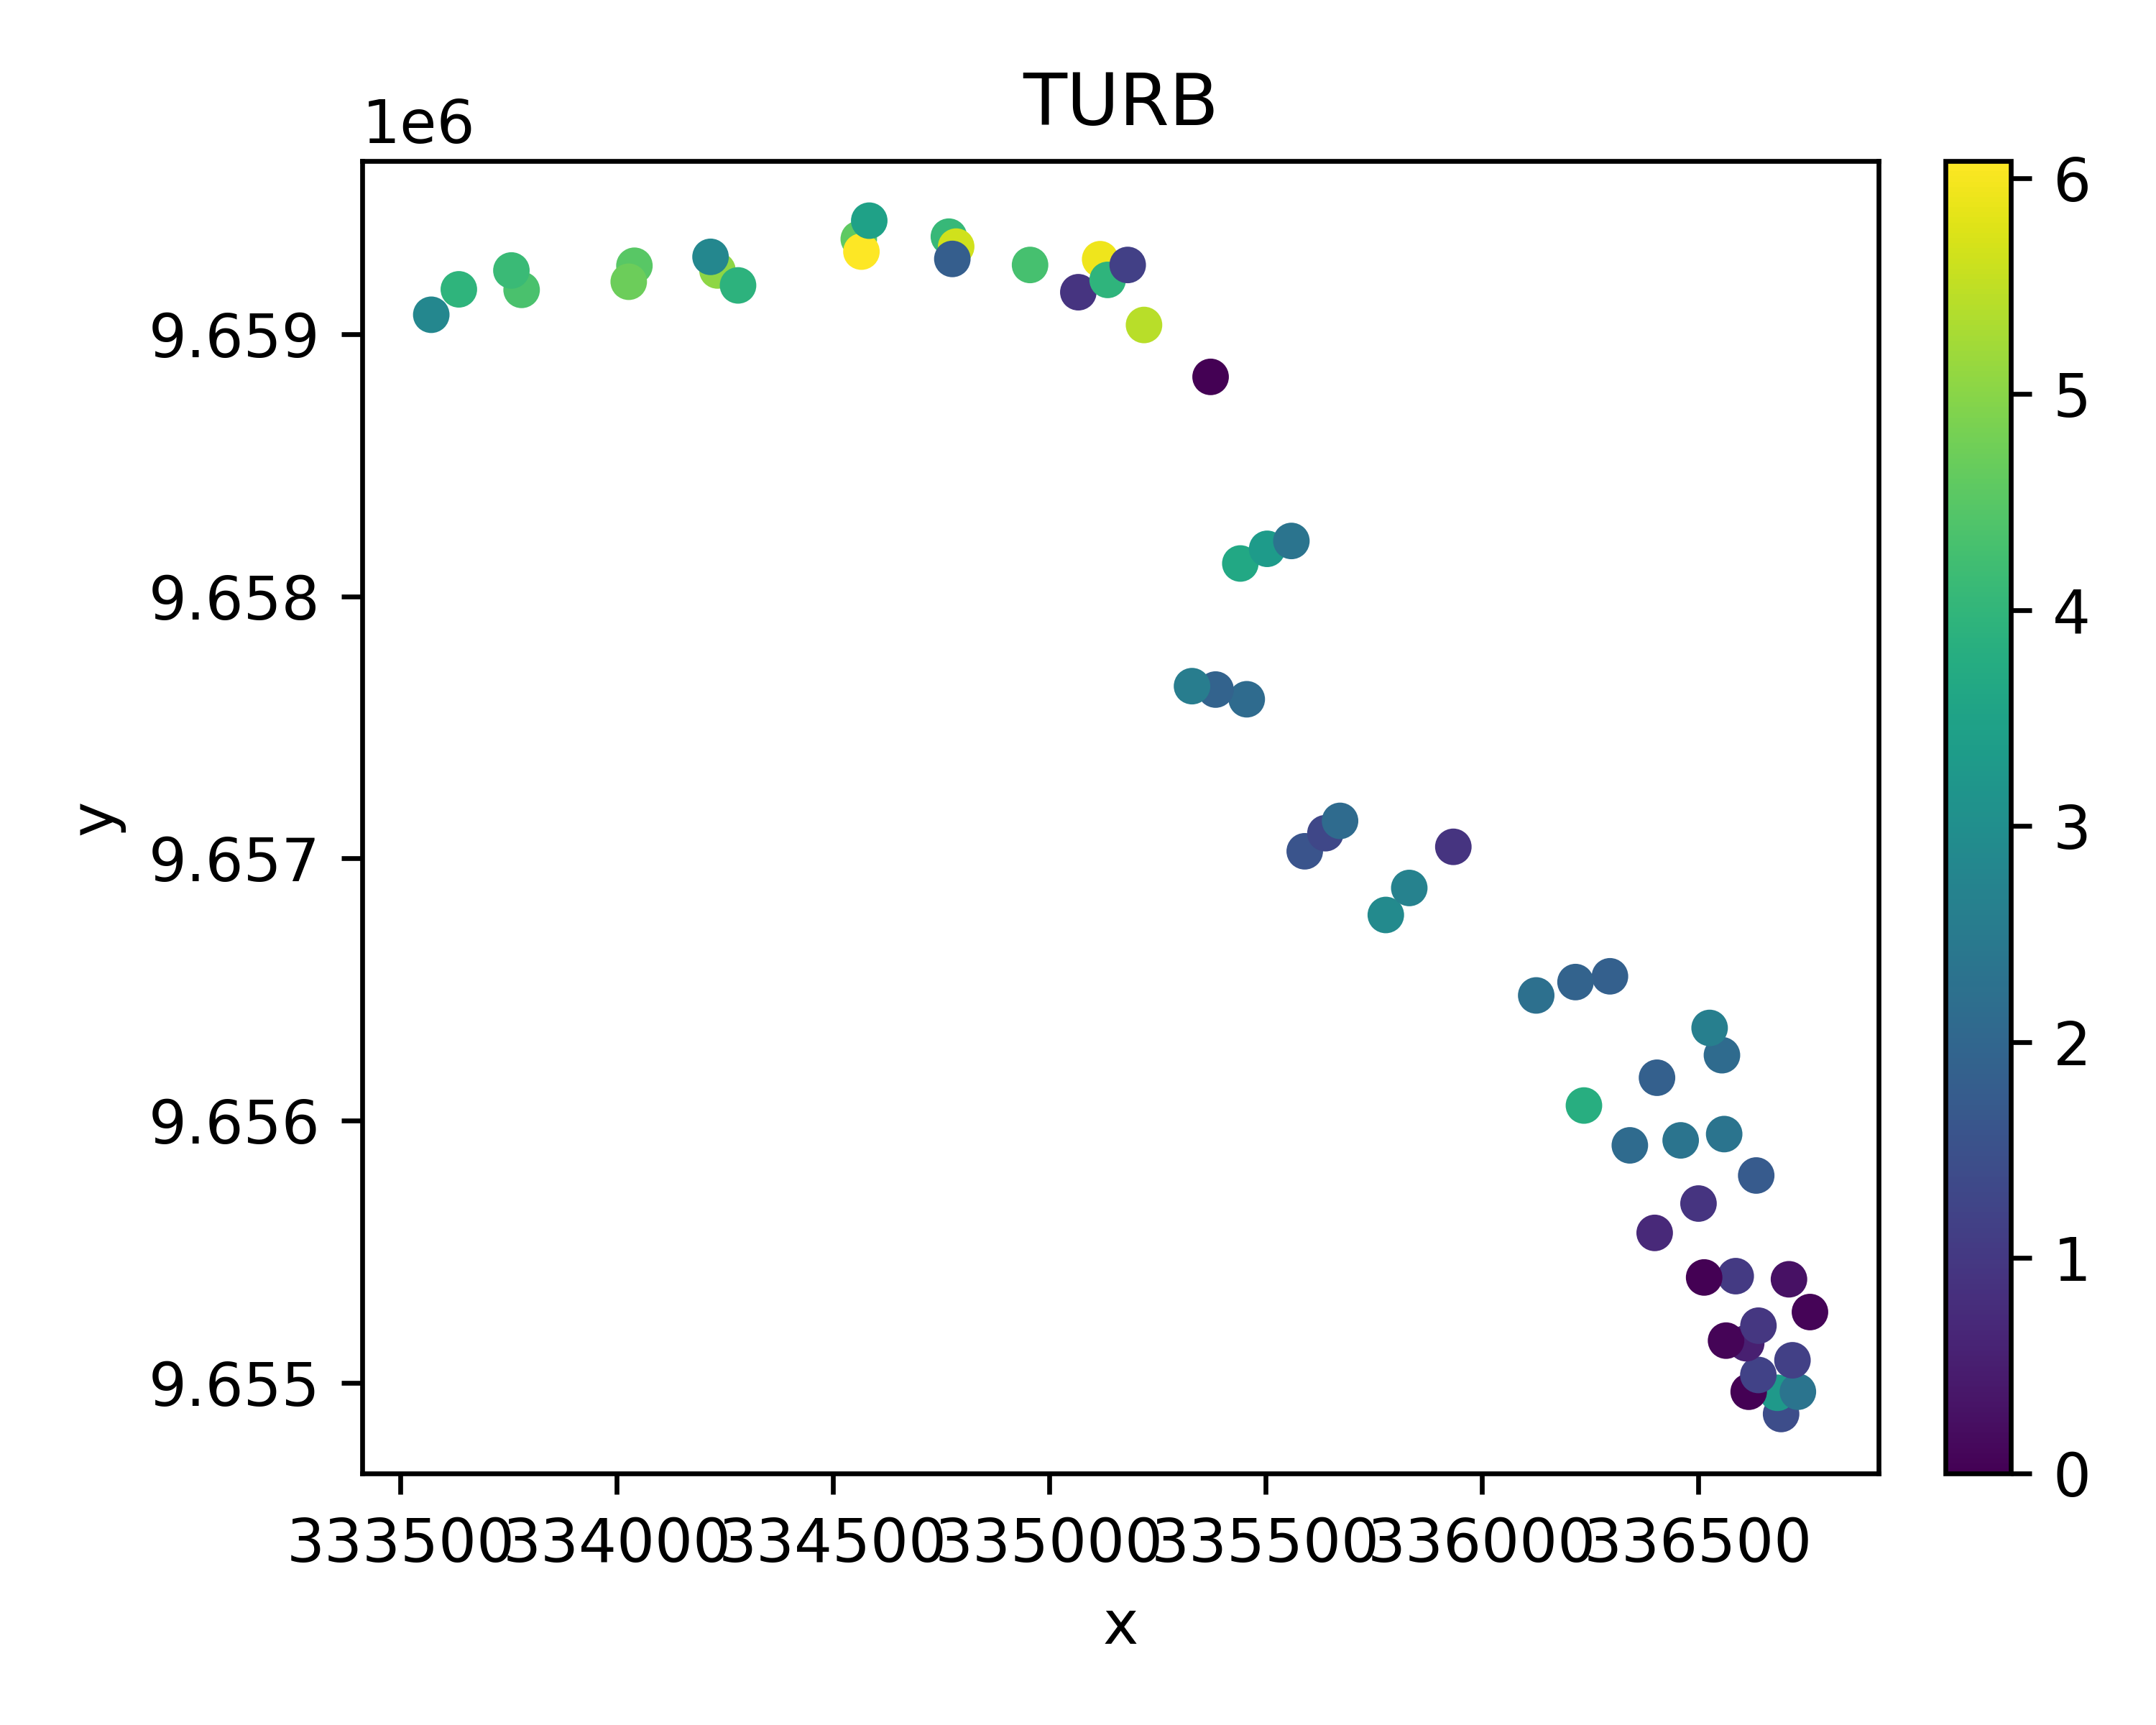
\includegraphics[width=\linewidth]{./figuras/map_TURB.png}
		\caption*{(b) Mapa espacial de turbidez}
	\end{minipage}
	\caption{Padrões espaciais de OD e turbidez.}
	\label{fig:mapas}
\end{figure}

Os mapas de OD e turbidez evidenciam heterogeneidade espacial, com áreas de maior turbidez e zonas
de OD relativamente reduzido. Essa variabilidade sugere influência local de processos físicos e
biogeoquímicos, justificando a necessidade de monitoramento em rede.

\begin{figure}[ht!]
	\centering
	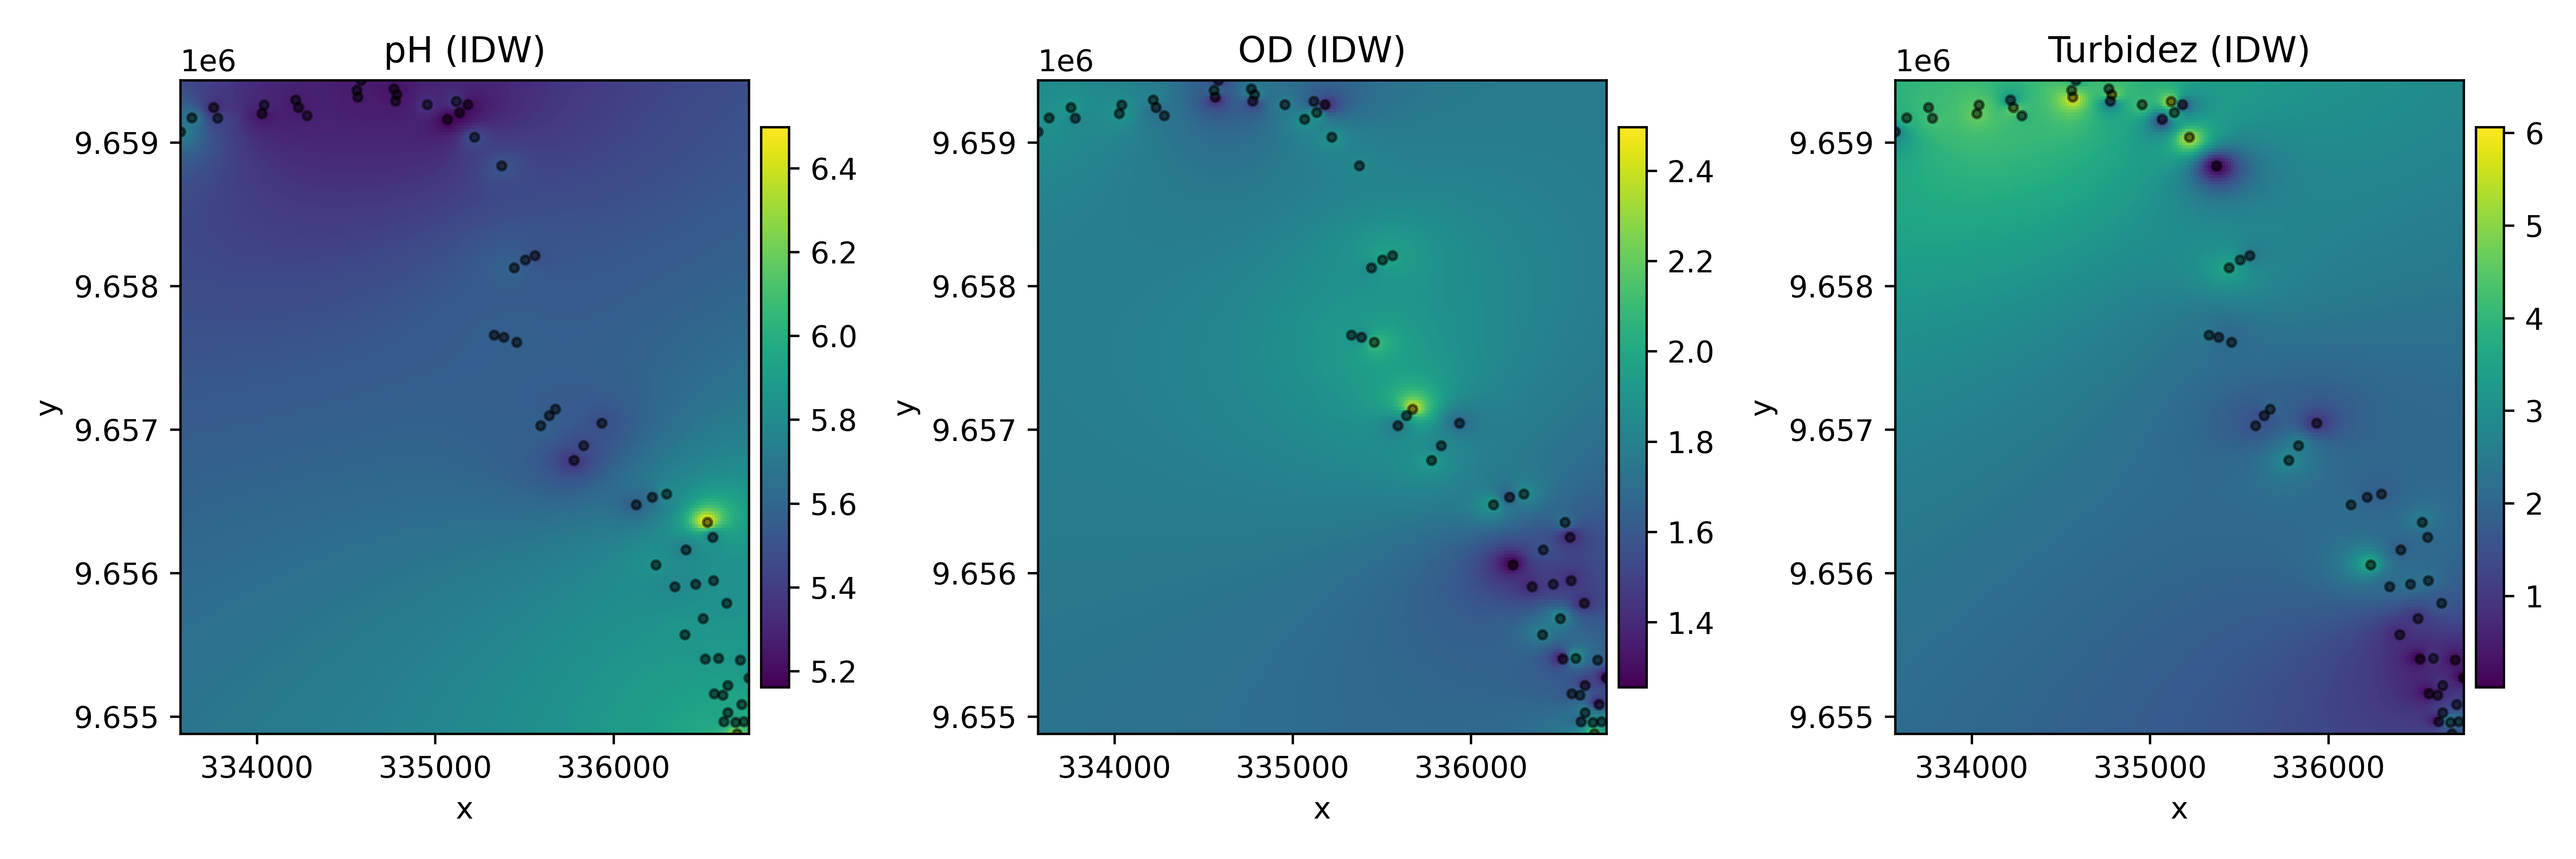
\includegraphics[width=0.98\textwidth]{./figuras/idw_combined.png}
	\caption{Superfícies interpoladas por IDW para pH, OD e turbidez a partir dos
	pontos amostrados.}
	\label{fig:idw}
\end{figure}

A Figura~\ref{fig:idw} apresenta as superfícies interpoladas (IDW) para pH, OD e turbidez, oferecendo
uma leitura contínua das variáveis a partir das medições pontuais. Observam-se gradientes espaciais
consistentes, permitindo identificar regiões com maior contraste entre os parâmetros.

\begin{figure}[ht!]
	\centering
	\begin{minipage}{0.32\textwidth}
		\centering
		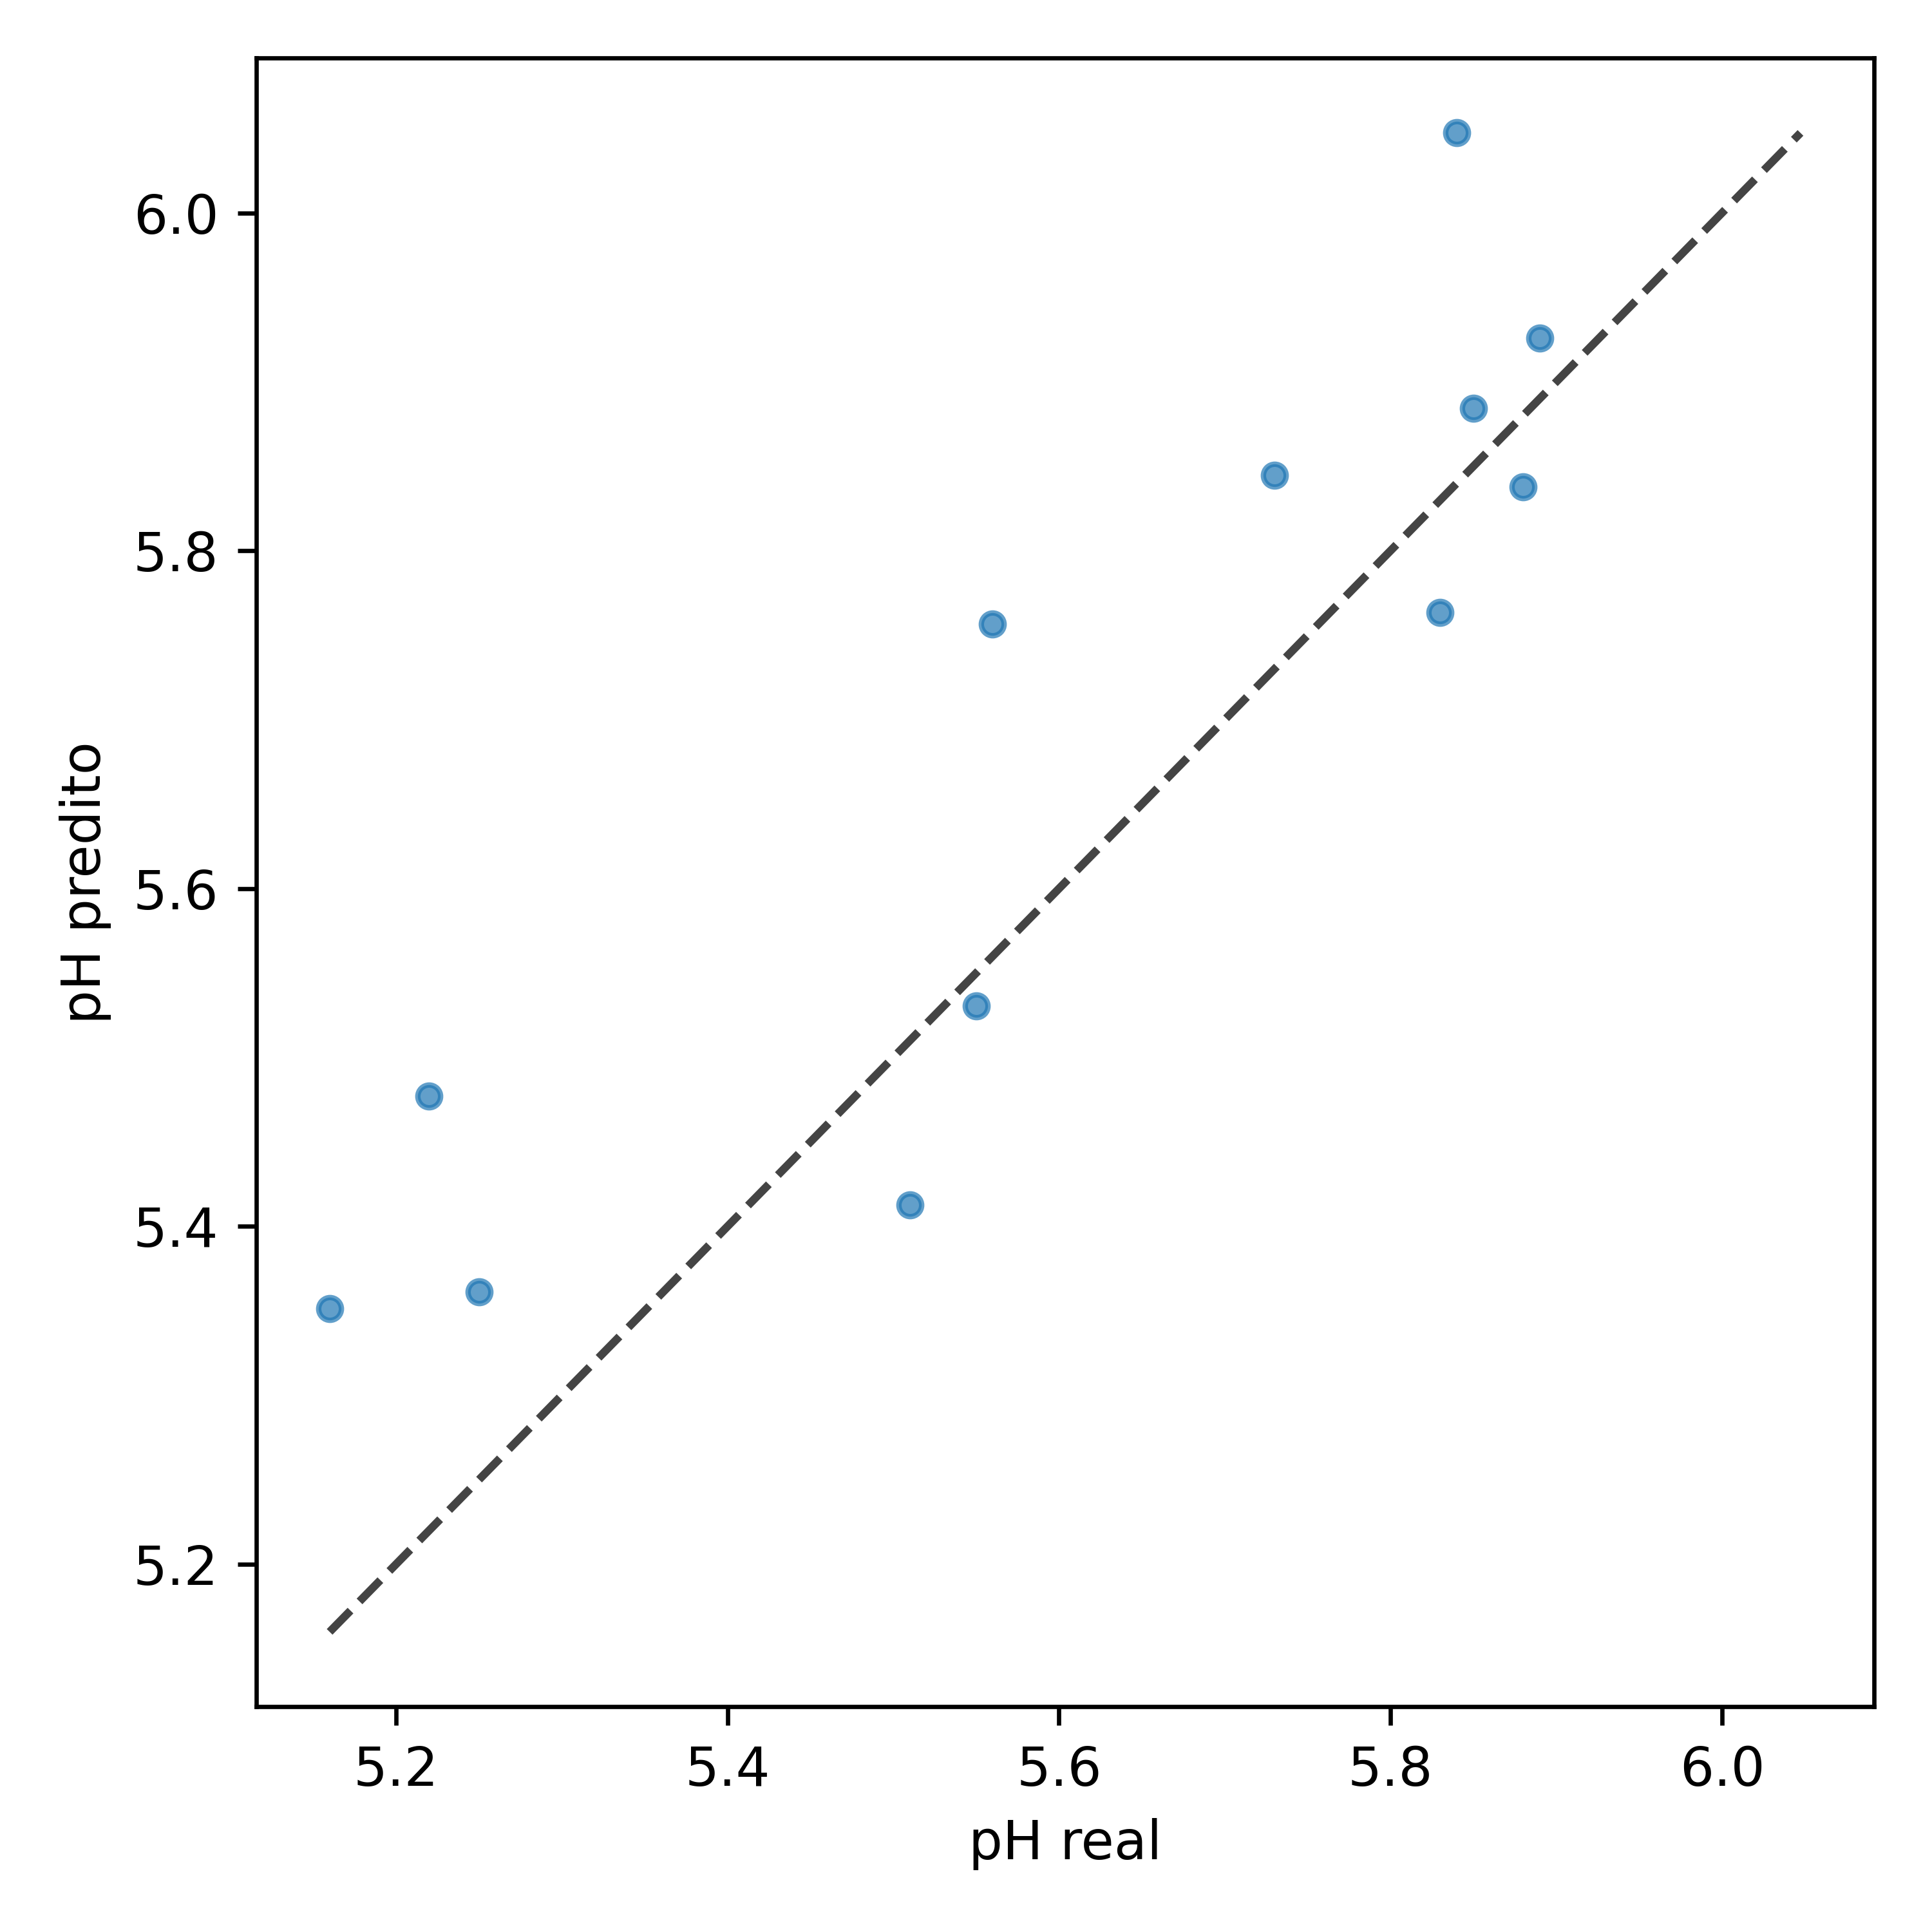
\includegraphics[width=\linewidth]{./figuras/pred_vs_real_pH_multi.png}
		\caption*{(a) pH}
	\end{minipage}\hfill
	\begin{minipage}{0.32\textwidth}
		\centering
		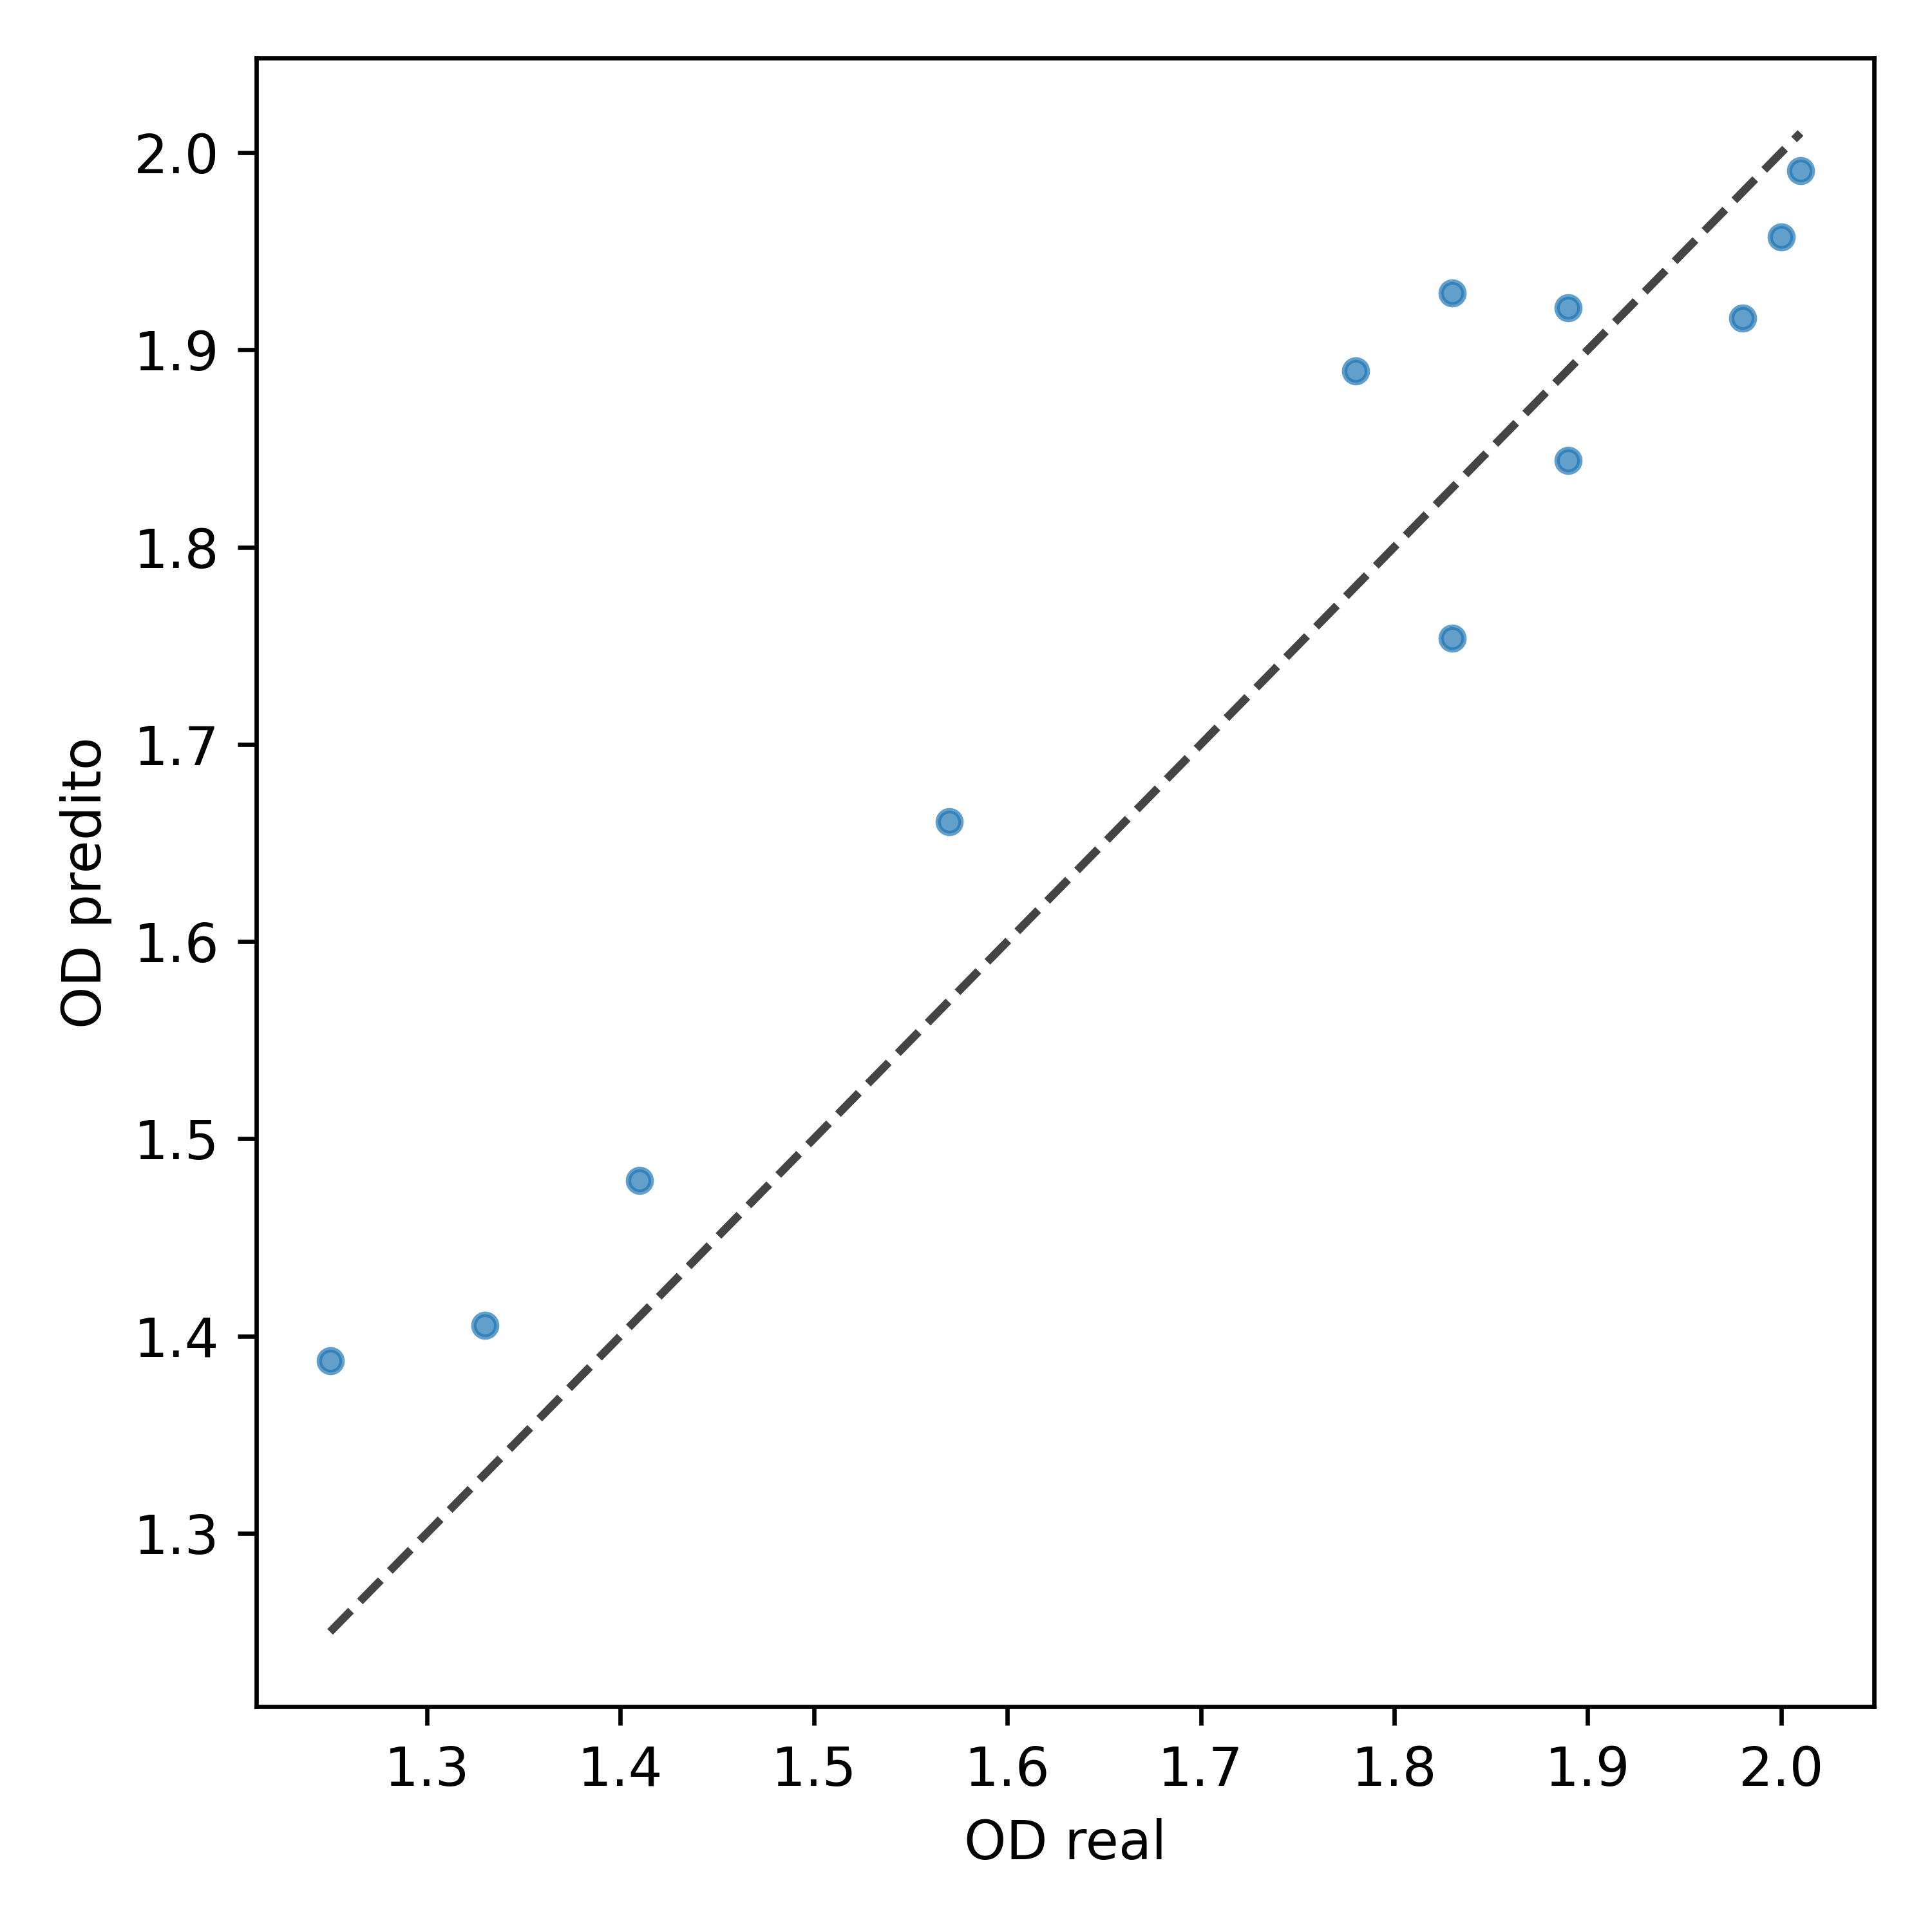
\includegraphics[width=\linewidth]{./figuras/pred_vs_real_OD_multi.png}
		\caption*{(b) OD}
	\end{minipage}\hfill
	\begin{minipage}{0.32\textwidth}
		\centering
		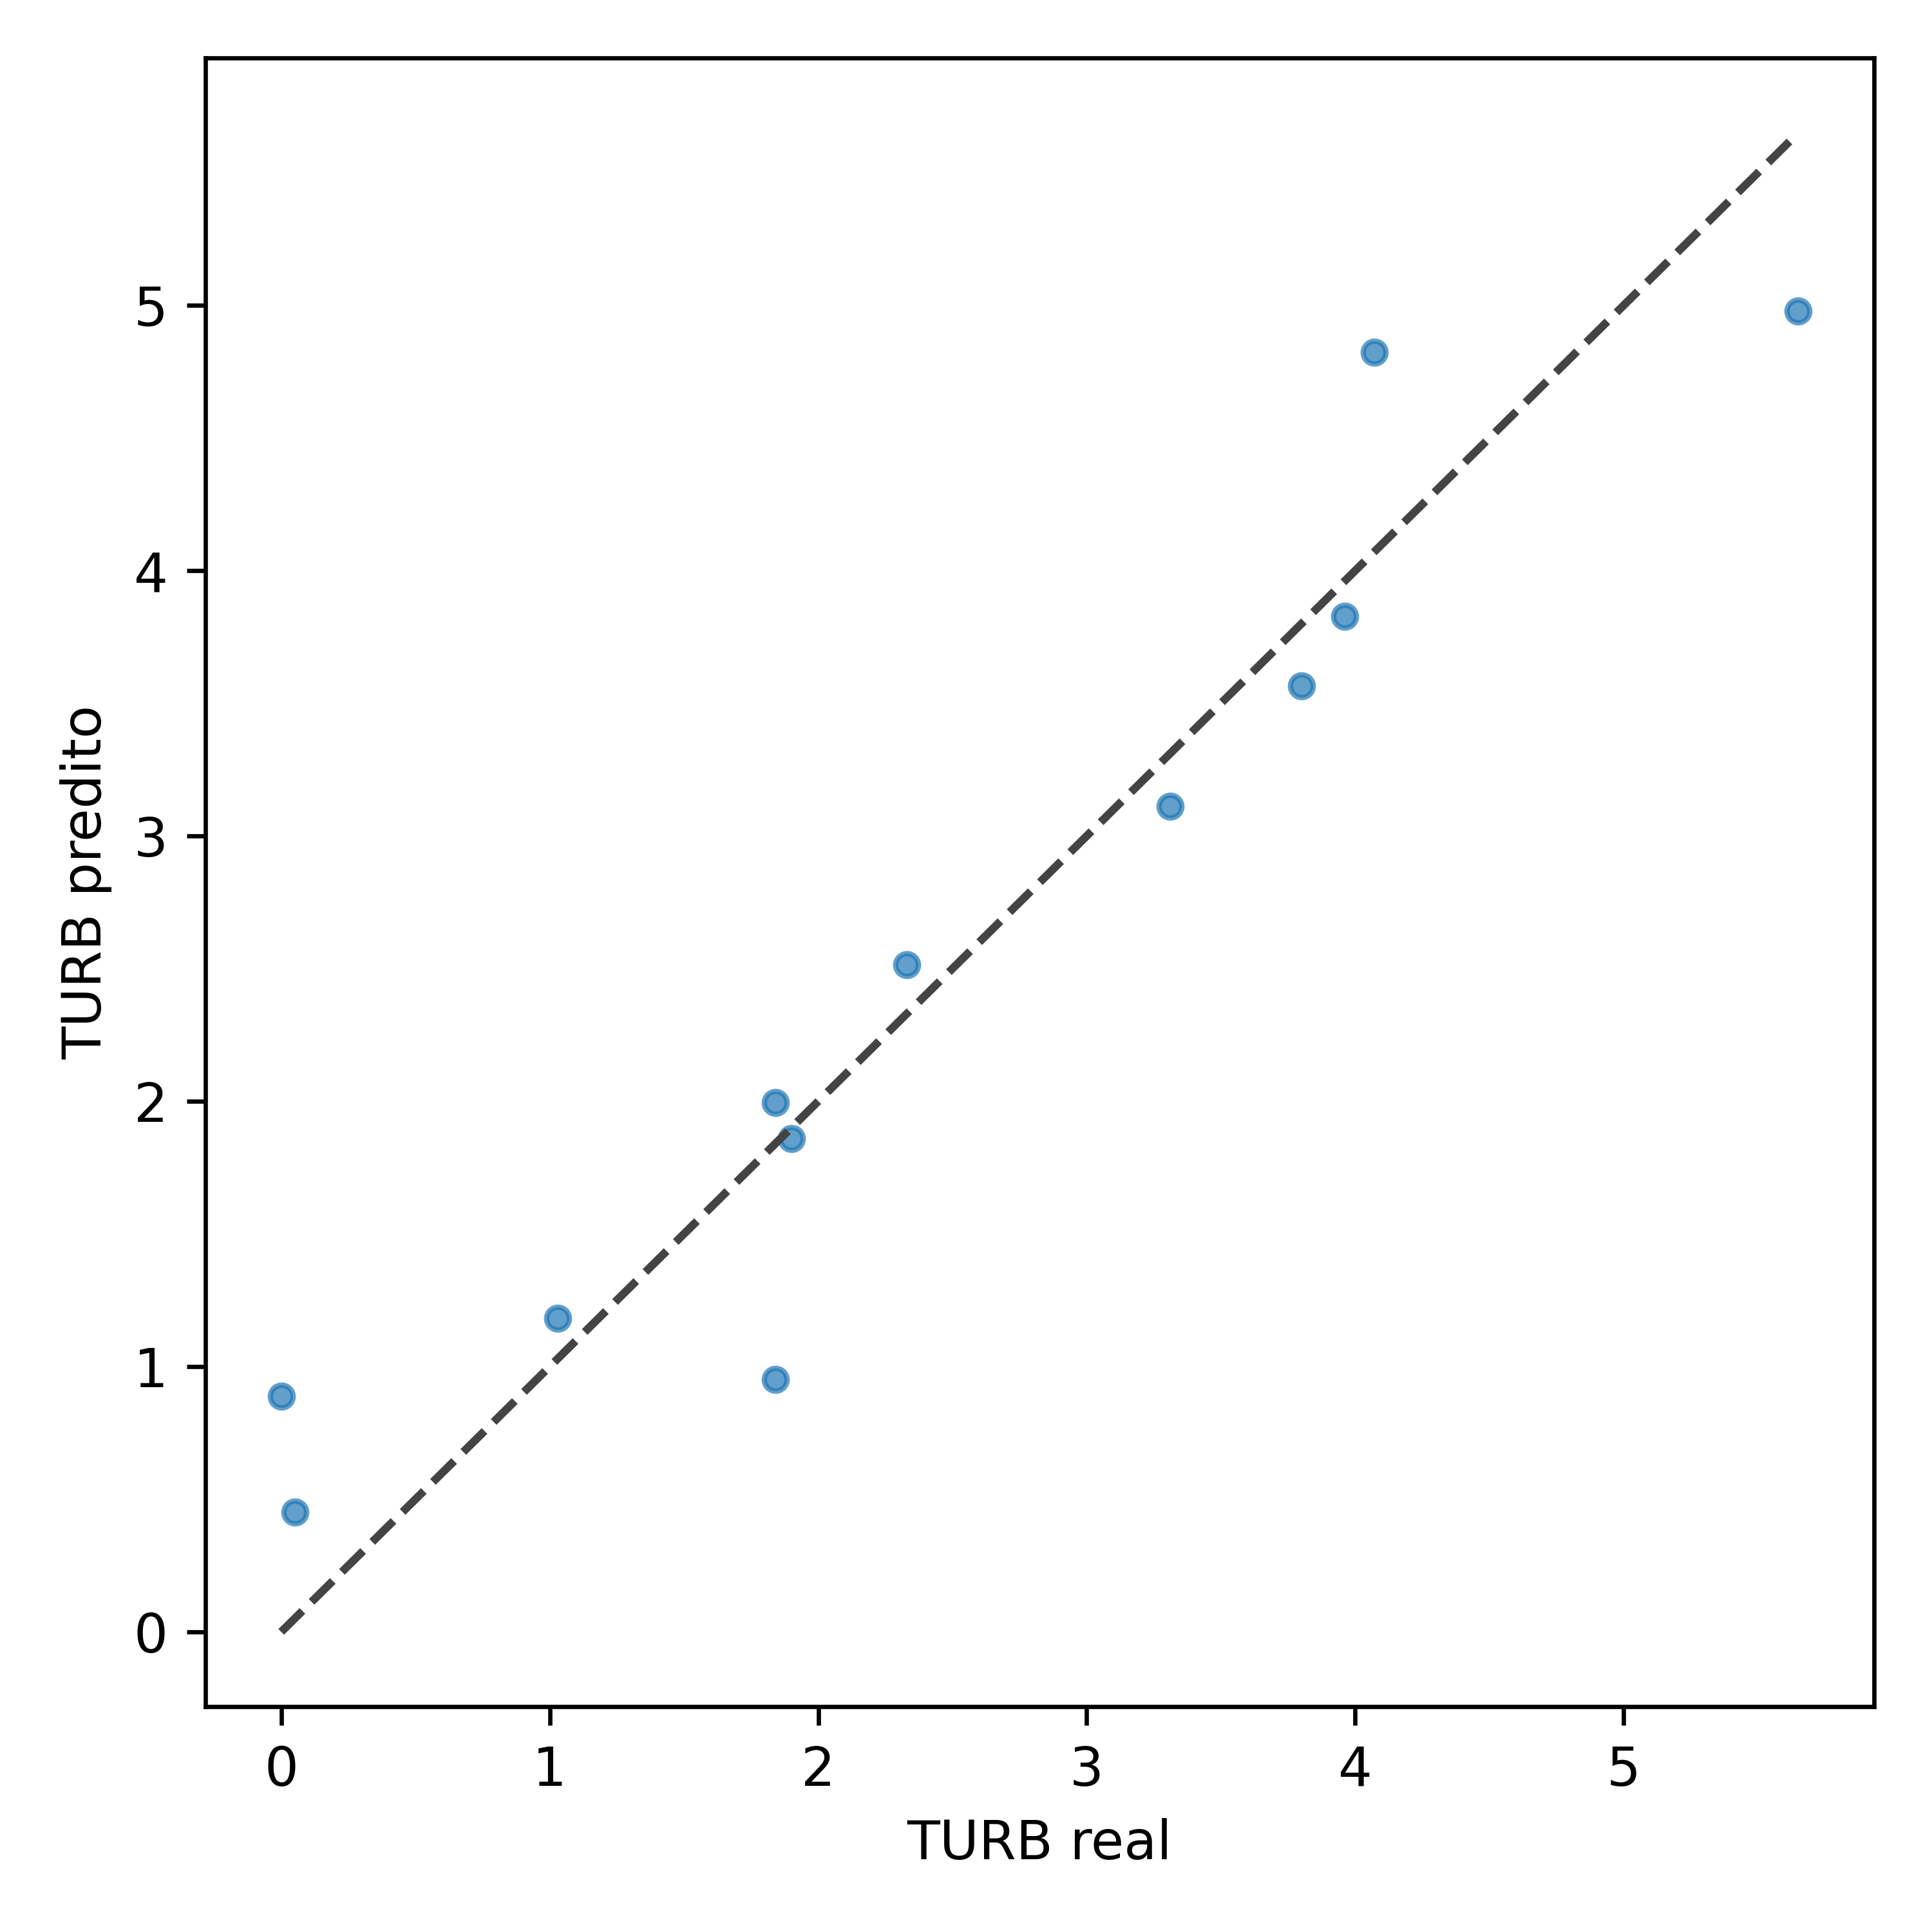
\includegraphics[width=\linewidth]{./figuras/pred_vs_real_TURB_multi.png}
		\caption*{(c) Turbidez}
	\end{minipage}
	\caption{Predito vs. real do modelo multimodal para pH, OD e turbidez.}
	\label{fig:multi_pred}
\end{figure}

Na Figura~\ref{fig:multi_pred}, o ajuste multimodal apresenta boa aderência para pH e OD, enquanto a
turbidez apresenta maior dispersão. Ainda assim, a tendência geral permanece alinhada à linha de
identidade, indicando capacidade preditiva satisfatória em múltiplas variáveis.

\begin{figure}[ht!]
	\centering
	\begin{minipage}{0.32\textwidth}
		\centering
		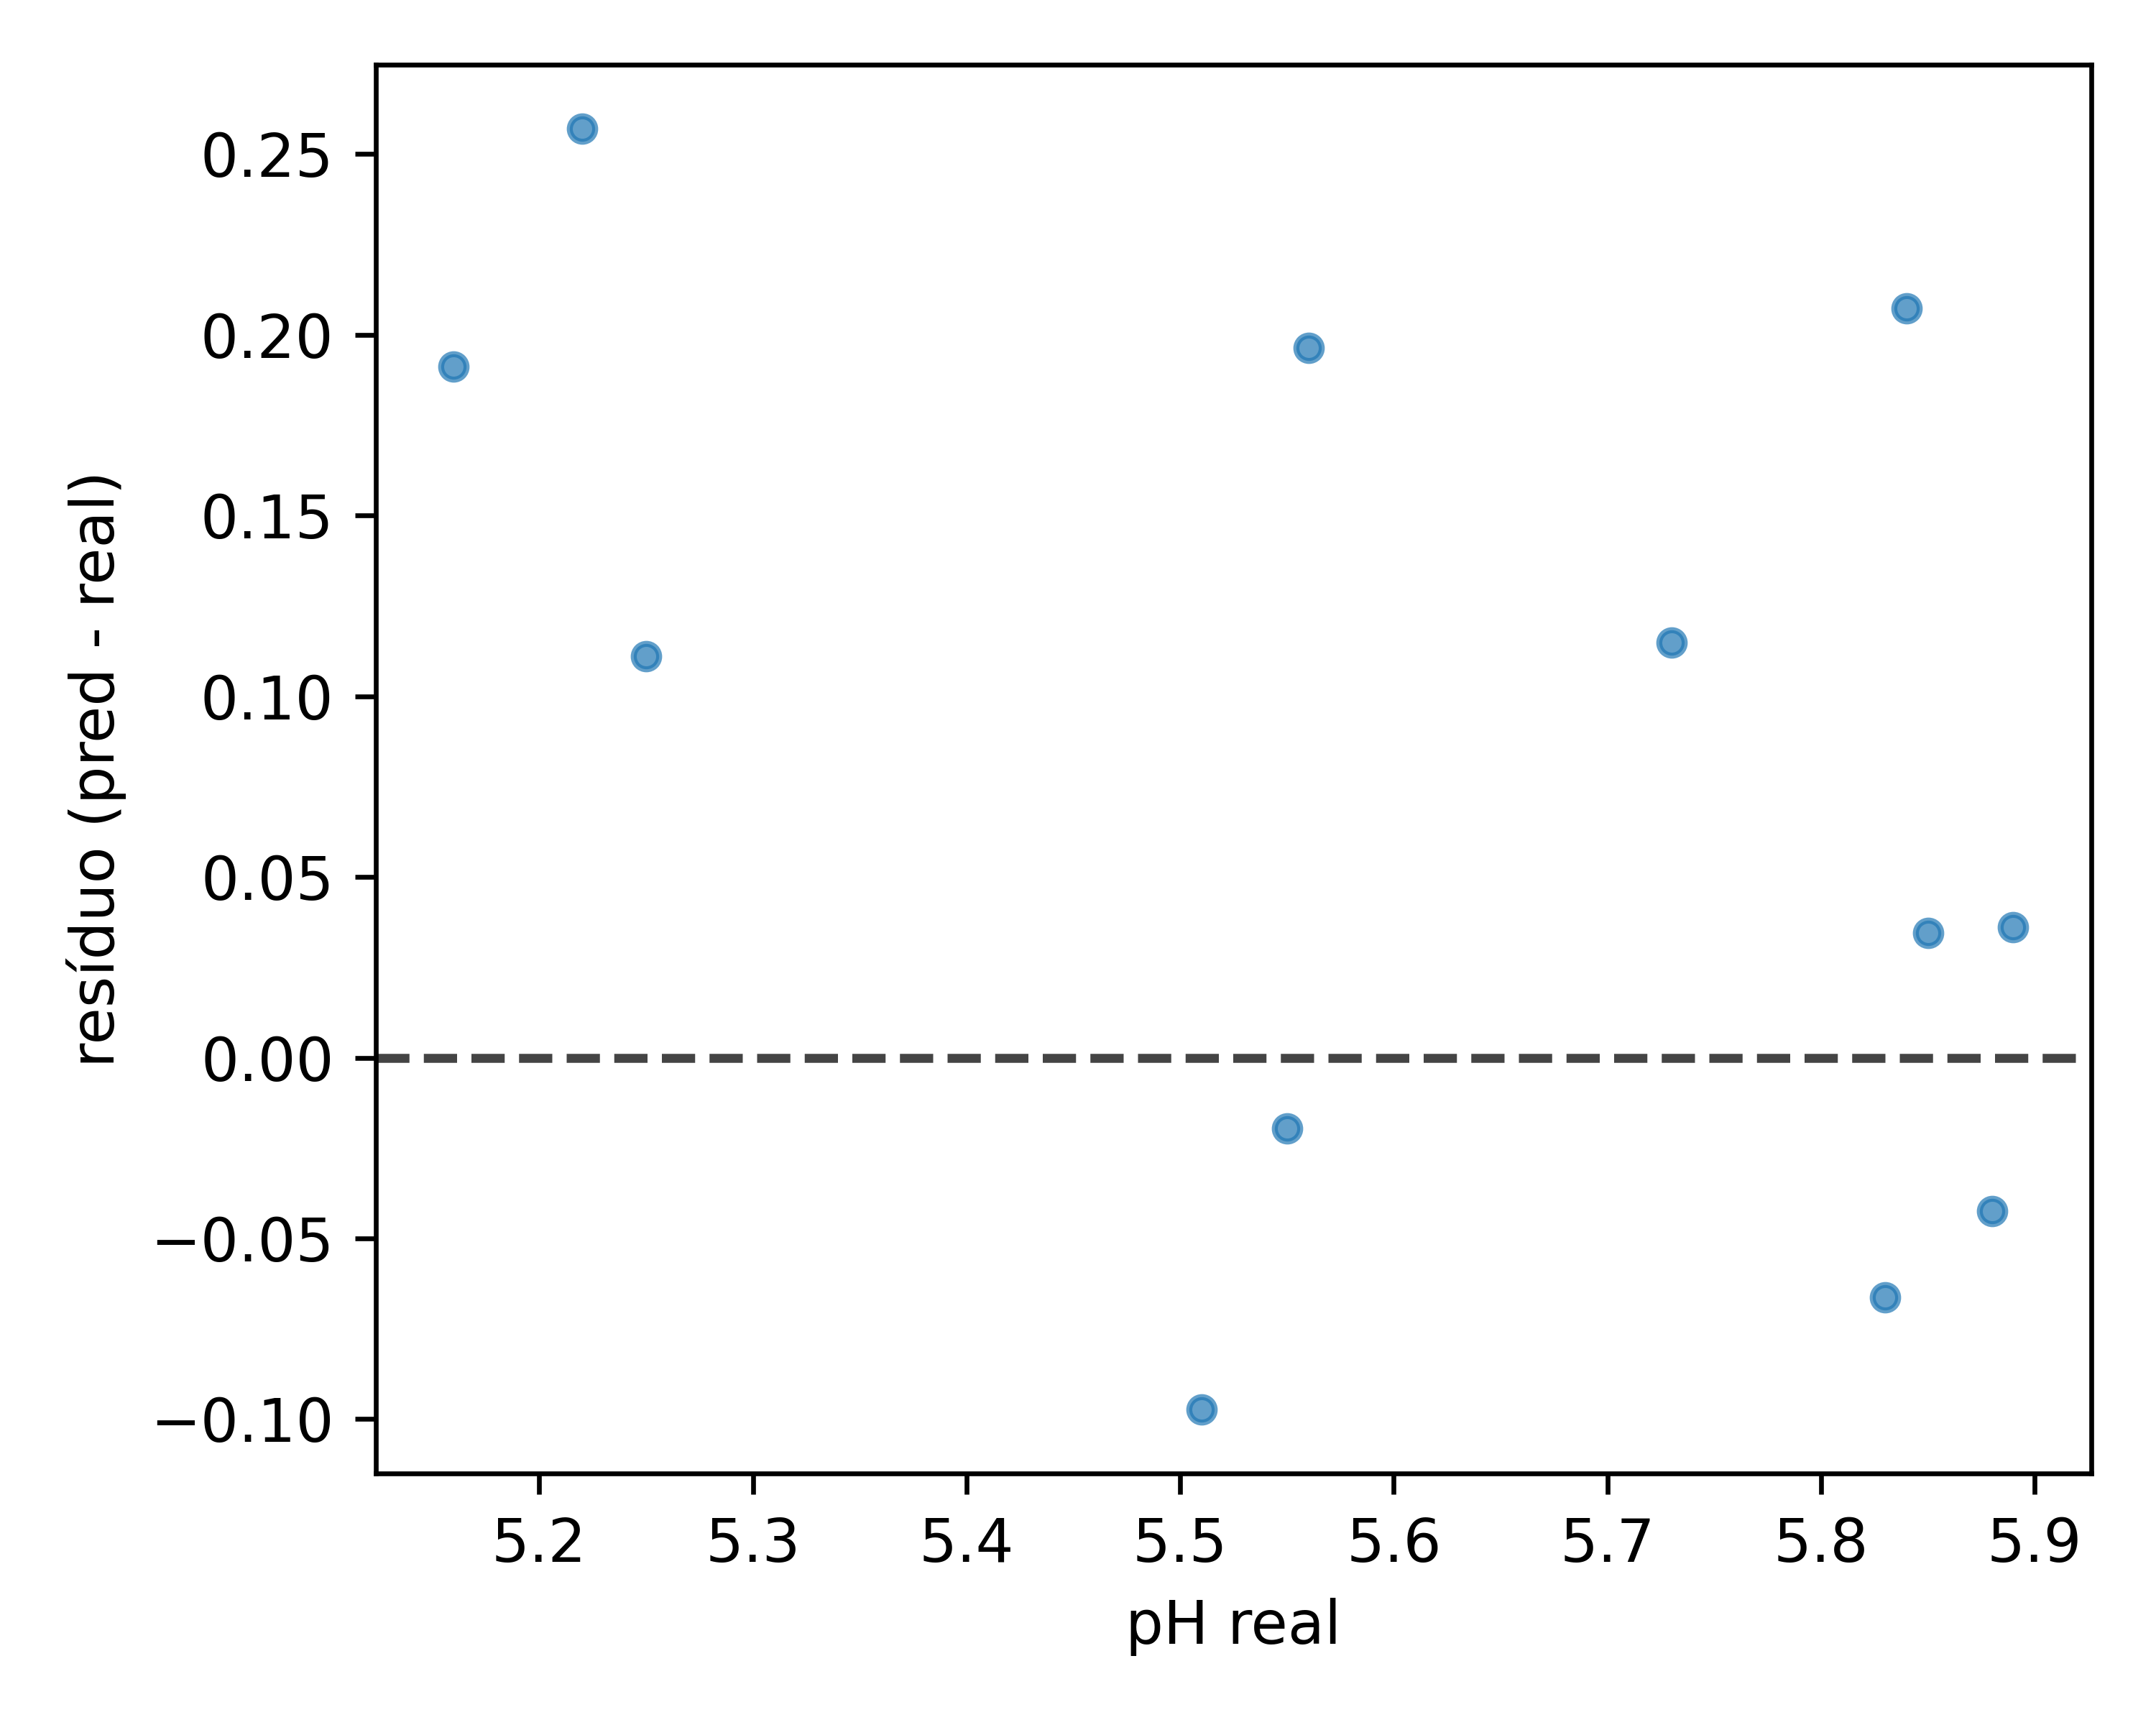
\includegraphics[width=\linewidth]{./figuras/residuals_pH_multi.png}
		\caption*{(a) pH}
	\end{minipage}\hfill
	\begin{minipage}{0.32\textwidth}
		\centering
		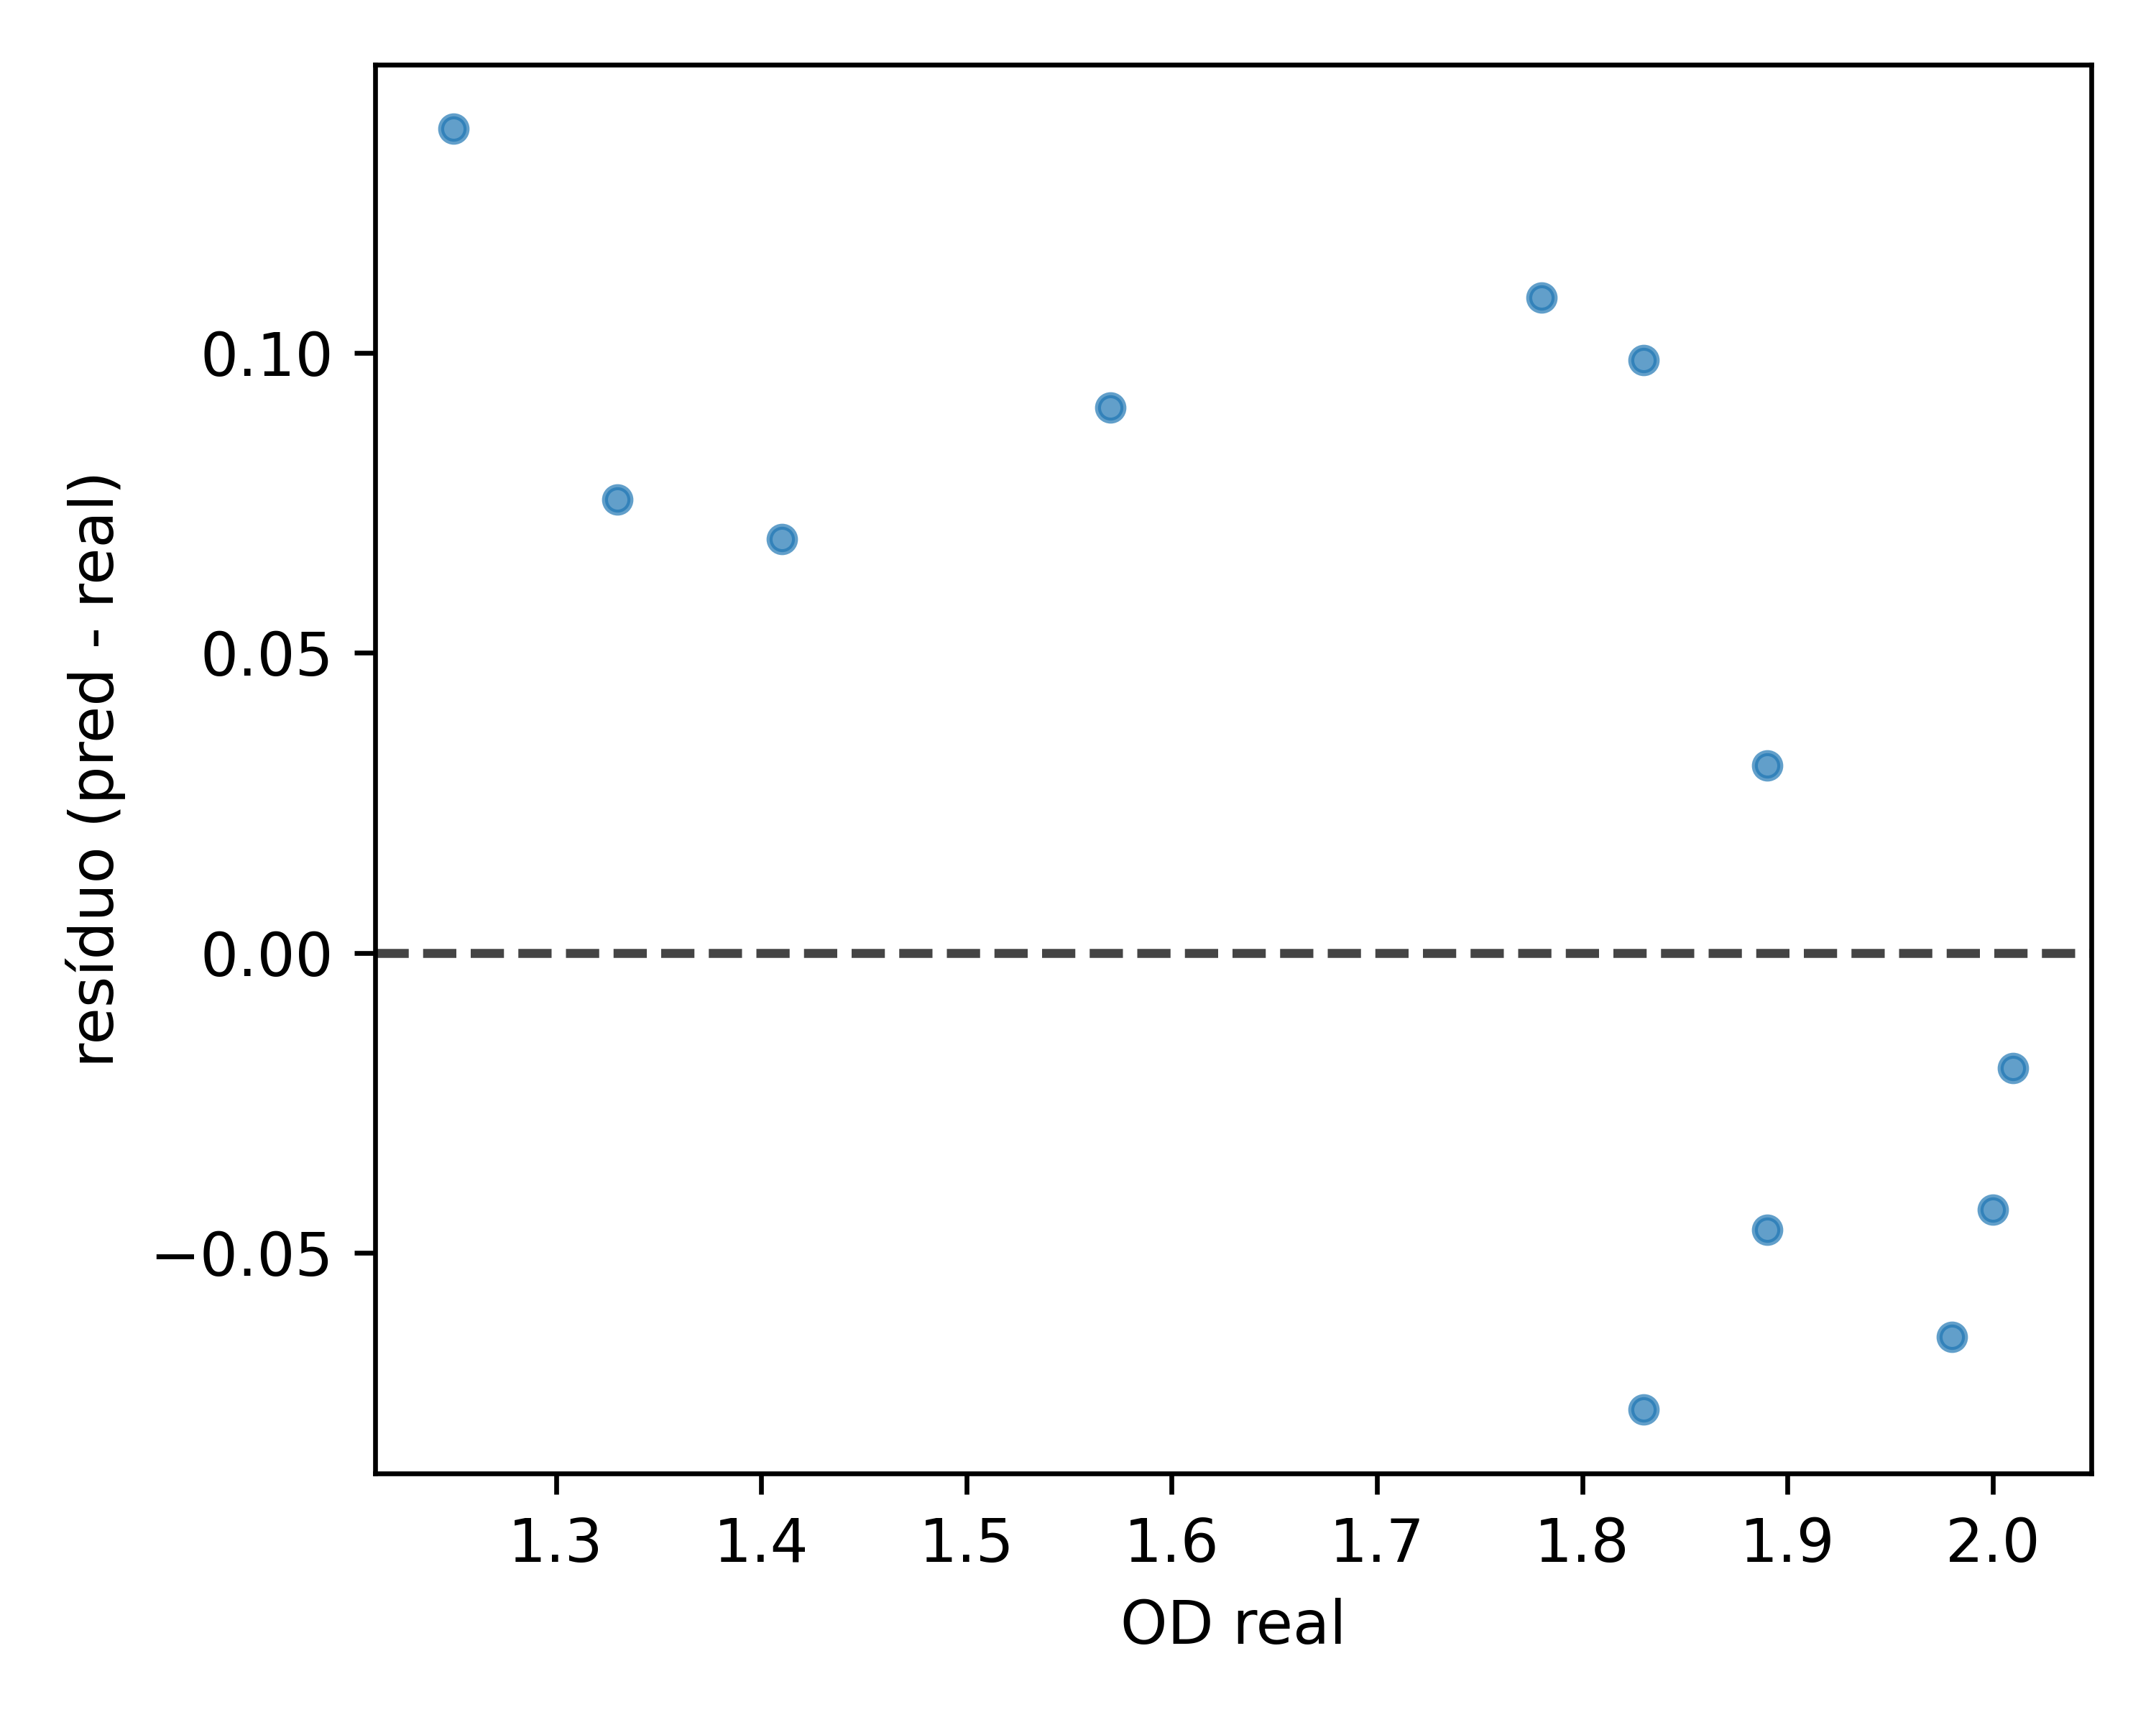
\includegraphics[width=\linewidth]{./figuras/residuals_OD_multi.png}
		\caption*{(b) OD}
	\end{minipage}\hfill
	\begin{minipage}{0.32\textwidth}
		\centering
		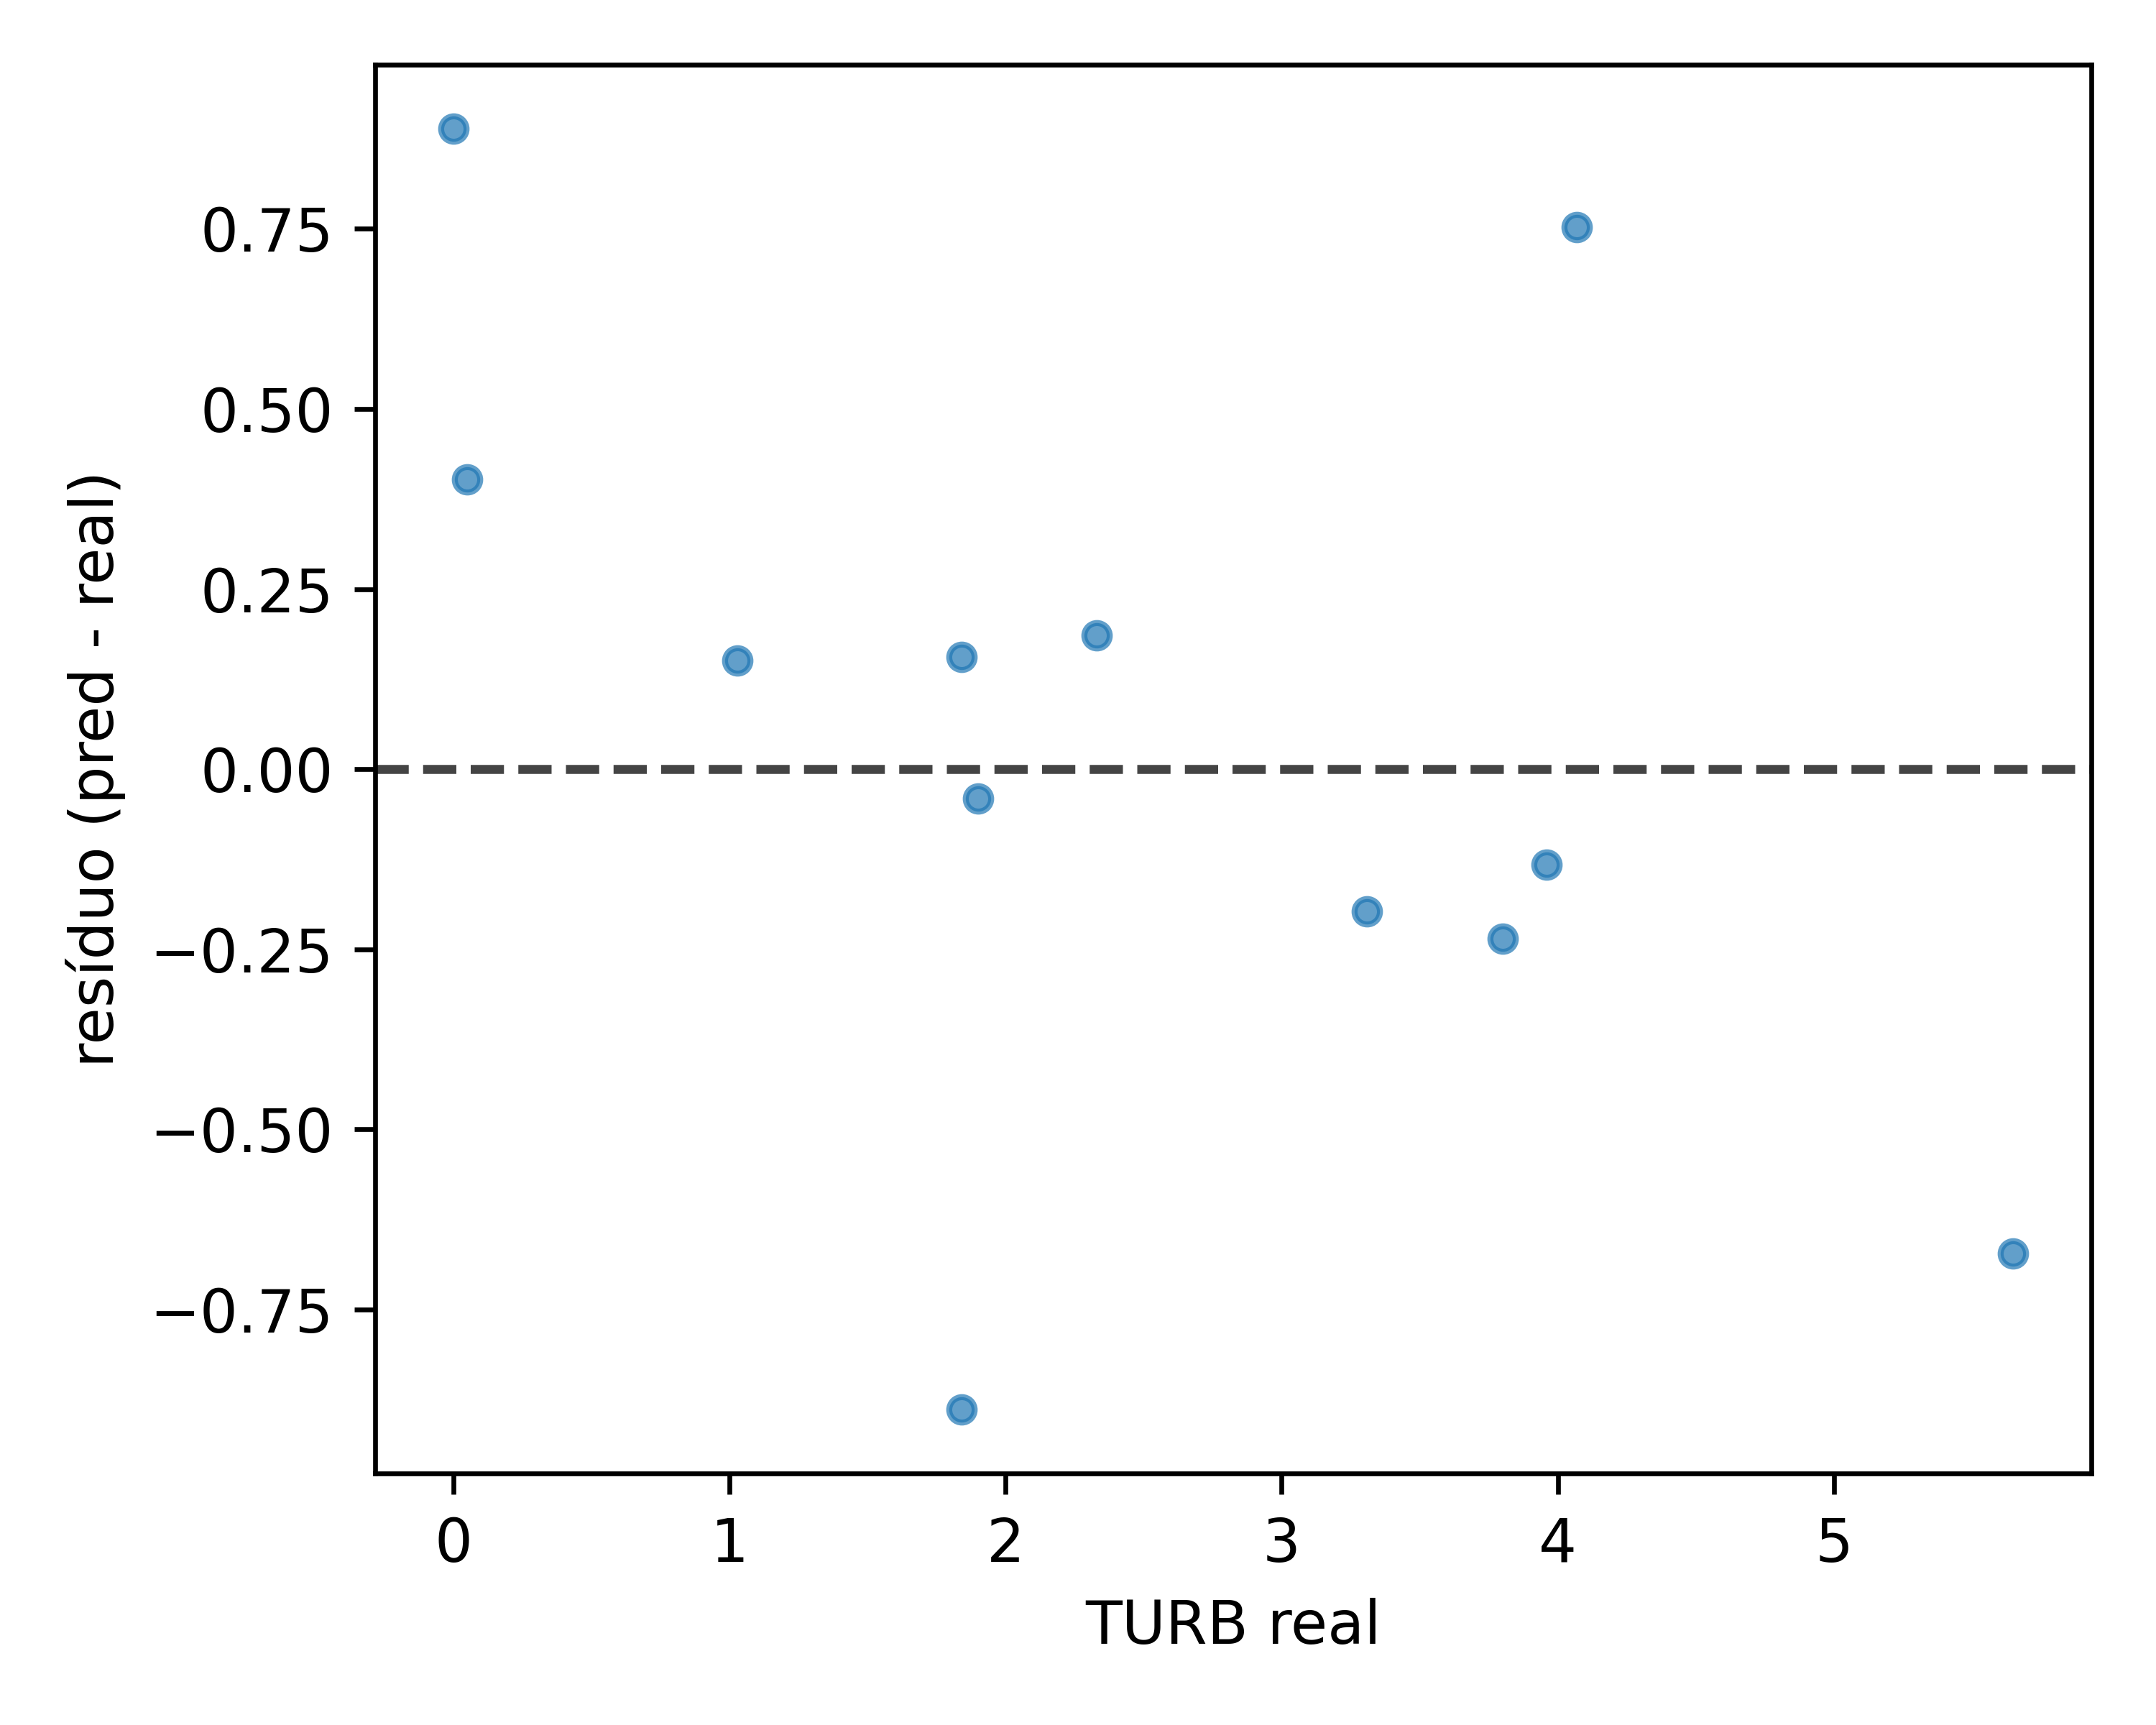
\includegraphics[width=\linewidth]{./figuras/residuals_TURB_multi.png}
		\caption*{(c) Turbidez}
	\end{minipage}
	\caption{Resíduos (predito - real) do modelo multimodal para cada variável.}
	\label{fig:multi_res}
\end{figure}

Os resíduos na Figura~\ref{fig:multi_res} se distribuem em torno de zero para pH e OD, sugerindo
ausência de viés sistemático relevante. Para turbidez, há maior variabilidade, indicando maior
dificuldade de modelagem e possível necessidade de mais dados ou calibração adicional.

\begin{figure}[ht!]
	\centering
	\begin{minipage}{0.48\textwidth}
		\centering
		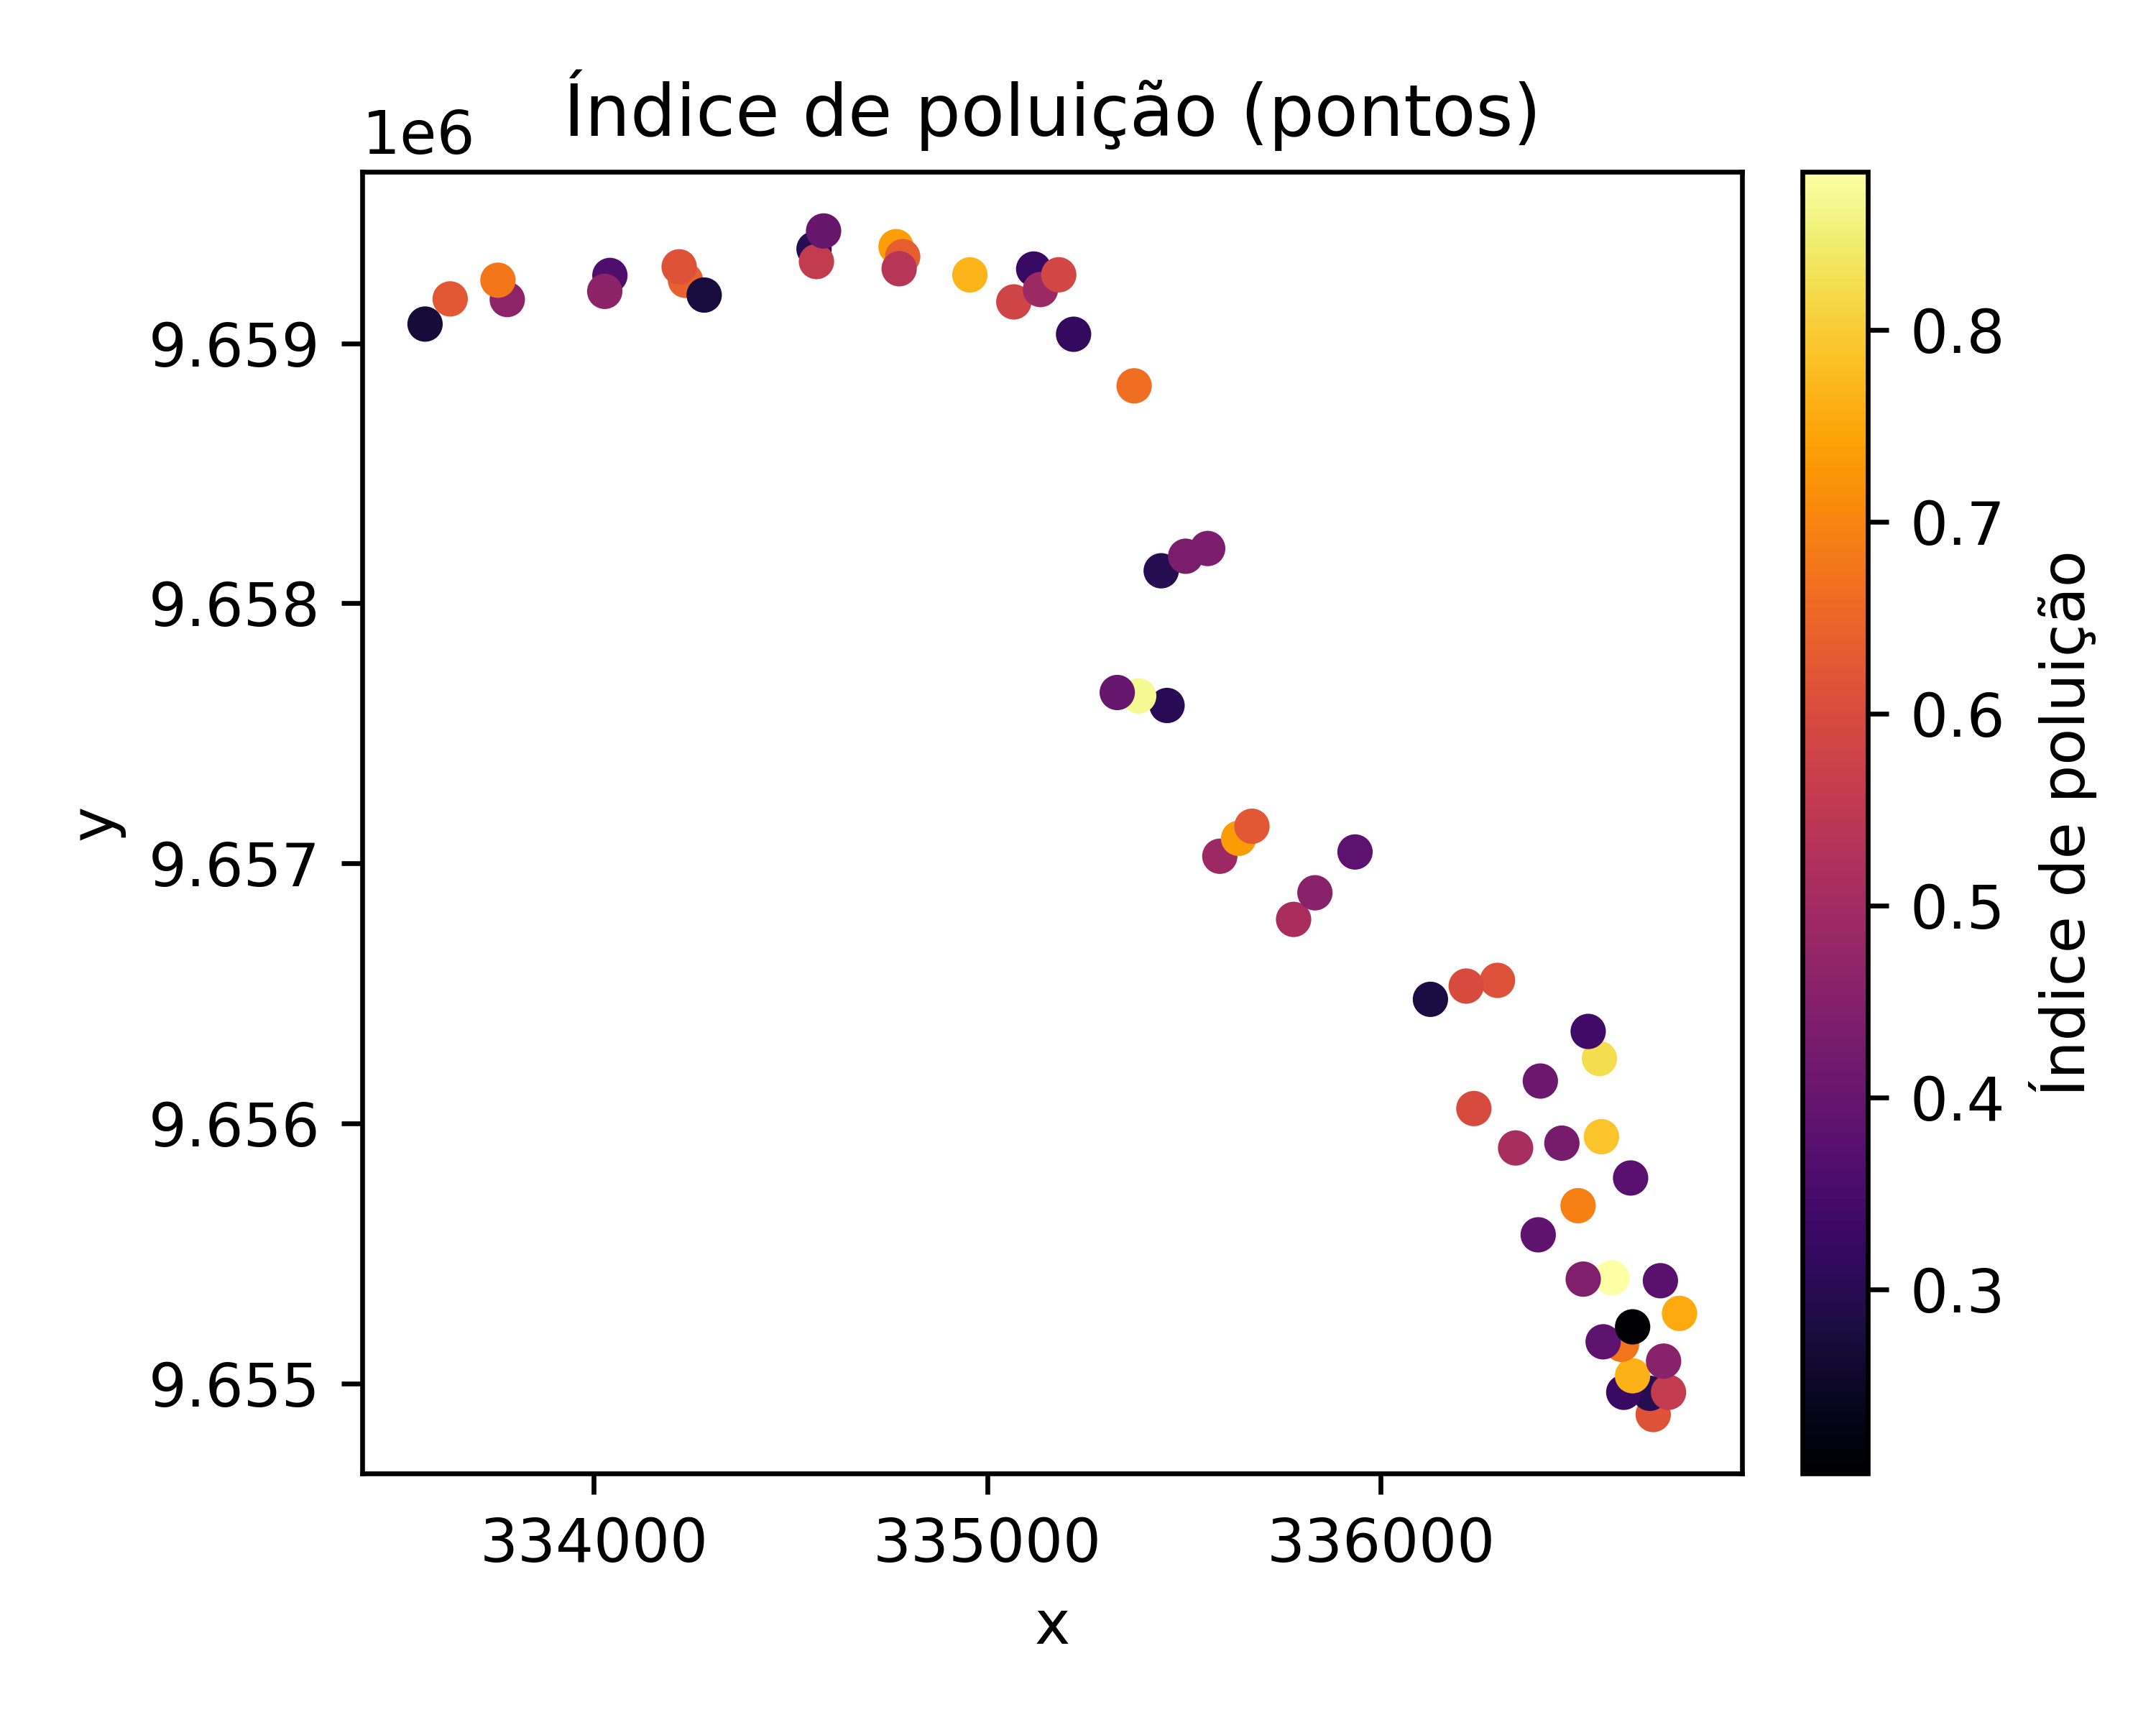
\includegraphics[width=\linewidth]{./figuras/pollution_scatter.png}
		\caption*{(a) Índice de poluição nos pontos}
	\end{minipage}\hfill
	\begin{minipage}{0.48\textwidth}
		\centering
		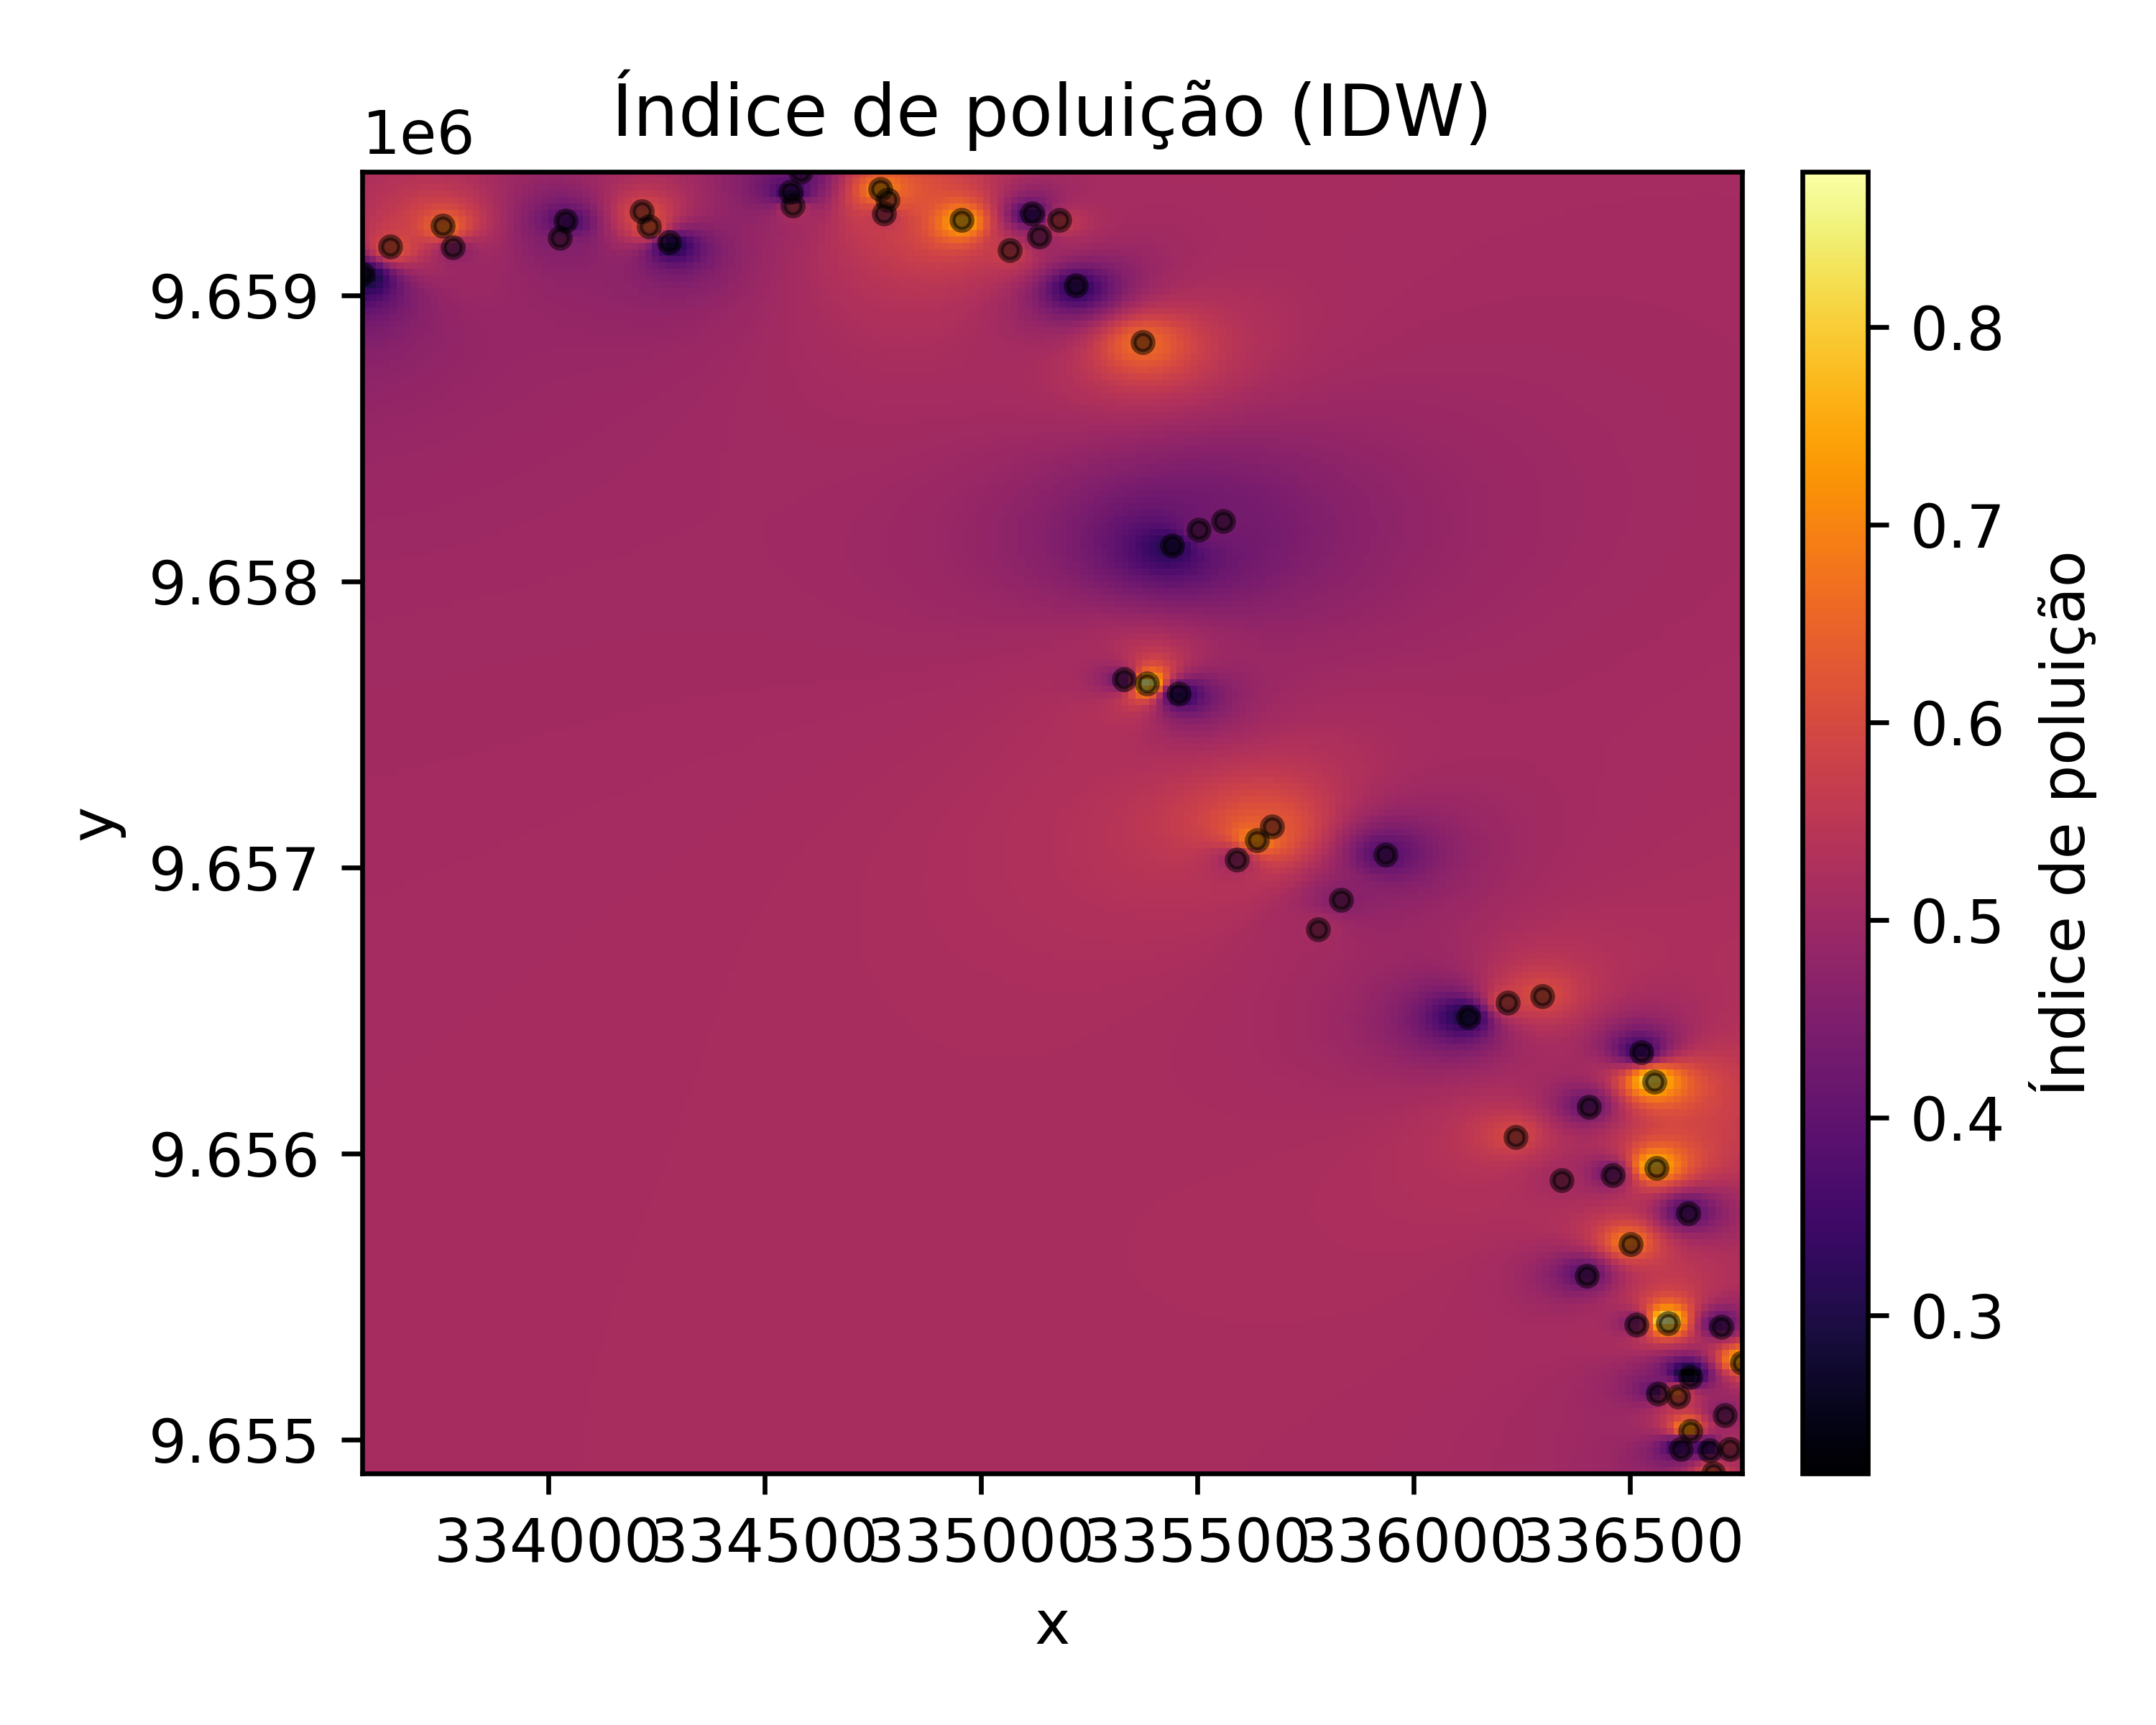
\includegraphics[width=\linewidth]{./figuras/pollution_idw.png}
		\caption*{(b) Mancha (IDW) do índice}
	\end{minipage}
	\caption{Estimativa espacial do índice de poluição composto a partir das
	predições multimodais.}
	\label{fig:pollution}
\end{figure}

A Figura~\ref{fig:pollution} apresenta o índice composto de poluição, combinando pH, OD e turbidez
em um único mapa. O gráfico de pontos evidencia locais com maior intensidade relativa, enquanto a
superfície interpolada por IDW permite visualizar a mancha de poluição estimada no corpo d’água.

\FloatBarrier
